\documentclass[11pt,a4paper]{amsbook}

\usepackage{amssymb}
\usepackage{amsmath}
\usepackage{graphicx}
\usepackage{enumitem}
\usepackage[english]{babel}
\usepackage[latin1]{inputenc}

\usepackage{Definitions}

\usepackage[a4paper,twoside,vscale=.7,hscale=.75,nomarginpar,hmarginratio=1:1]{geometry}

\usepackage{hyperref}
\usepackage{pdfpages}
\usepackage{xcolor}

\usepackage{algorithm}
\usepackage{algorithmic}

\definecolor{orangegood}{RGB}{226,147,2}
\definecolor{bluegood}{RGB}{0,92,155}
\hypersetup{
    colorlinks=true,
    linkcolor=bluegood,
    linktoc=page,
    citecolor=bluegood
}

\newtheorem{theorem}{Theorem}[chapter]
\newtheorem{lemma}[theorem]{Lemma}
\newtheorem{proposition}[theorem]{Proposition}
\newtheorem{corollary}[theorem]{Corollary}

\theoremstyle{definition}
\newtheorem{definition}[theorem]{Definition}
\newtheorem{example}[theorem]{Example}
\newtheorem{xca}[theorem]{Exercise}

\theoremstyle{remark}
\newtheorem{remark}[theorem]{Remark}

\numberwithin{section}{chapter}
\numberwithin{equation}{chapter}

\newcommand{\from}{\colon}
\newcommand{\ev}{\mathbf{E}}
\newcommand{\xhat}{\hat{x}}
\newcommand{\prob}[1]{\mathop{\mathrm{Pr}}[#1]}

\newcommand{\note}[1]{\textit{\color{cyan}Note: #1}}
\newcommand{\projon}[2]{\operatorname{Proj}_{#1}(#2)}
\newcommand{\proj}[1]{\operatorname{Proj}(#1)}
\setcounter{tocdepth}{1}

\newcommand{\simplex}{\Delta}
\newcommand{\grad}{\nabla}

\usepackage[round]{natbib}
\setcitestyle{authoryear,open={(},close={)}}

\linespread{1.1}

\addto\captionsenglish{\renewcommand{\bibname}{References}}


\begin{document}
\frontmatter

\begin{titlepage}
    \begin{center}
        
\includegraphics[width=5cm]{figures/eth-logo}\hfill
        
\includegraphics[width=5cm]{figures/las-logo}
        \vspace{4cm}

        {\Huge
            \textbf{Consistent Online Optimisation}
        }
        
        \vspace{2cm}
        {\large
            \textsc{Mohammad Reza Karimi Jaghargh}
        }

        \vspace{2cm}
        {\large
            \textbf{Master Thesis}\\
        }
        
        \vspace{.5cm}
        Computer Science Department\\
        Learning and Adaptive Systems Group\\
        ETH Z\"urich
        
        \vspace{2cm}
        {\large
            \textbf{Supervisor}\\[.5cm]
            Prof. Dr. Andreas Krause
        }
        \vfill
        \today
        
    \end{center}
\end{titlepage}

\setcounter{page}{0}
\clearpage\thispagestyle{empty}\mbox{}\clearpage
\title{Consistent Online Optimisation}
%    Information for first author
\author{Mohammad Reza Karimi Jaghargh}
%    Address of record for the research reported here
\address{ETH Z\"urich, Switzerland}
%    Current address
\email{mkarimi@ethz.ch}
\maketitle

\begin{abstract}
    Modern online learning algorithms achieve low (sublinear) regret in a variety of diverse settings. These algorithms, however, update their solution at every time step. While these updates are computationally efficient, the very requirement of frequent updates makes the algorithms untenable in practical applications where the change of solution is costly. In this work, we develop online learning algorithms that update their solution a sublinear number of times. We give a meta-algorithm based on non-homogeneous Poisson processes that gives a smooth trade-off between the regret and frequency of updates. Empirically, we show that in our two real-world examples, one can significantly reduce updates at a minimal increase in the regret.
\end{abstract}

\setcounter{page}{4}
\tableofcontents

\mainmatter

\chapter{Introduction}
Bandit, expert learning, and convex optimisation algorithms have revolutionised online learning, and low regret algorithms are now known for a multitude of diverse settings. Whether the examples are drawn from a distribution, are chosen by an adversary,  come annotated with additional context, or are selected from arbitrary convex domains, there are efficient algorithms that achieve sublinear, $o(T)$, regret after $T$ timesteps. 

One characteristic of these algorithms is that they rarely stick with playing the same action repeatedly, instead, continually exploring new decisions. While this exploration is necessary to achieve low regret, the constant switching between actions can have adverse effects in practice, both from a systems standpoint, and user interface design.  On the systems side,  a lot of switching can wreak havoc on caches, and incur additional latency in the processing of results.  At the same time, most users prefer a sense of predictability, or {\em consistency} in their interactions with the system, and overly dynamic systems add to the overall cognitive load.  

In this work, we investigate the trade-off between the consistency cost (defined as the number of times the algorithm changes its action), and the regret achieved by the algorithm. We show that a simple modification of classic online gradient descent approaches leads to a smooth trade-off between the two goals. At a high level, we achieve this by probabilistically deciding whether to keep playing the same action, or perform an update step. Importantly, we can do this with \emph{constant} additional overhead---the additional computation needed to decide the probability of whether to update takes only constant time. 

Finally we note that our algorithm can be easily extended to more complex settings. For instance, in Section~\ref{sec:submodapplication} we show how to extended our technique to solve the consistent online submodular maximisation problem, and in Chapter~\ref{chap:rftl} we show similar results hold for regularised online algorithms.

\section{Related Work}
Online Convex Optimisation is a very active research topic in online learning with many beautiful results~\citep{DBLP:journals/tit/MerhavOSW02}. Perhaps the closest to our setting is the work on learning with memory~\citep{DBLP:journals/tit/MerhavOSW02}. 
In this problem, the adversary is oblivious to the algorithm's choices but the loss that the algorithm incurs depends on the current and the recent choices of the algorithm. 
Interestingly, although the setting is different from ours, the algorithms introduced to solve this problem have non-trivial consistency guarantees. Often, the algorithms  are based on a blocking technique~\citep{DBLP:journals/tit/MerhavOSW02} that divides the rounds in blocks and allows only a constant number of switches per block. 
In turn, this technique automatically guarantees also to have a limited consistency cost, but with higher regret\footnote{The regret of this technique is $O(T^{2/3})$ and the consistency cost is of $O(T^{1/3})$.}. 
This result was later improved by~\cite{DBLP:journals/tit/GyorgyN14} using the Shrinking Dartboard framework introduced by~\cite{DBLP:conf/colt/GeulenVW10}, but unfortunately their technique is limited to the expert setting. Recently, \cite{DBLP:conf/nips/AnavaHM15} proposed a new algorithm that obtains near optimal bounds for the Online Convex Optimisation setting in the counterfactual feedback model where the algorithm knows the loss that it would have incurred had it played any sequence of $m$ decisions in the previous rounds. 
Our results are incomparable with these because our algorithm does not assume to have access to counterfactual feedback. Furthermore, it is simpler and can be easily extended to handle more complex settings like the consistent online submodular maximisation problem.

A related area to ours is metrical task systems (MTS). The player's goal is to minimise the movement (in a metric space) plus the costs she recieves, while holding a plausible \emph{competitive ratio}, \ie, the ratio of the cost of the algorithm relative to the cost of the optimal offline algorithm on a worst-case sequence. Important problems in this field include the $k$-server problem \citep{manasse1990competitive,bubeck2017} and convex chasing problem \citep{argue2019nearly}. 

Another area of work that is closely related to ours is research in online algorithms with recourse. In this setting, one seeks better online algorithms to compute optimal or approximate solutions for combinatorial problems by allowing the algorithm to make a limited number of changes to the online solution. 
This concept is very close to the notion of consistency that we consider in this paper. The first problem that received a lot of attention in this area is the classic online Steiner tree problem introduced by~\cite{DBLP:journals/siamdm/ImaseW91} for which it is possible to design better algorithms by allowing a small recourse as shown in several papers \citep{DBLP:journals/siamcomp/GuG016, DBLP:conf/soda/GuptaK14, DBLP:conf/stoc/LackiOPSZ15, DBLP:journals/siamcomp/MegowSVW16}. The concept of recourse has been applied to other classic optimisation problems as online scheduling \citep{DBLP:journals/algorithmica/AndrewsGZ99, DBLP:journals/algorithmica/EpsteinL14, DBLP:journals/algorithmica/PhillipsW98, DBLP:journals/mor/SandersSS09, DBLP:conf/esa/SkutellaV10}, online flow \citep{DBLP:conf/soda/GuptaKS14, DBLP:journals/jal/Westbrook00}, online matching \cite{DBLP:conf/soda/BernsteinHR18} and online set cover \citep{DBLP:conf/stoc/GuptaK0P17}. Very recently, \cite{DBLP:conf/icml/LattanziV17} introduced the notion of consistency in online algorithms for machine learning and studied the consistent online clustering problem.

\section{Contributions}
The main contributions of this thesis can be summarised as follows:
\begin{itemize}
    \item We present the first truly online learning algorithms, capable of dealing with large action sets, that trade-off the frequency with which the solution is updated and the final regret achieved.
    \item We provide explicit regret and consistency trade-offs for Online Gradient Descent, Online Submodular Maximisation, and Regularised Follow The Leader algorithms.
    \item We evaluate our theoretical results on two real-world datasets and show that our proposed method are compatible with, and mostly better than, our theoretical guarantees.
\end{itemize}

Much of this work is presented in \citet{karimi2019}, a joint work with Andreas Krause from ETH Z\"urich, Silvio Lattanzi and Sergei Vassilvitskii from Google, recently published in the 22\textsuperscript{nd} International Conference on Artificial Intelligence and Statistics (AISTATS 2019). Specifically, chapters 1, 3 and 5 are mainly based on the aforementioned paper.

\section{Acknowledgements}
I am grateful for having Prof. Andreas Krause as my supervisor in this research. His constant support and enlightening ideas and excellent guidance were crucial for the success of this work. I also thank Silvio Lattanzi and Sergei Vassilvitskii for our collaboration on this problem and our useful discussions. 

I am also very happy that I have been hosted by the Learning and Adaptive Systems (LAS) group during this research. Specifically, I shall thank Rita Klute for her kind help throughout the process of the thesis.

\chapter{Preliminaries}
Here we bring the preliminaries to this work, including some remarks about online learning, Poisson processes, and submodularity.

\section{Online Learning}
Many prediction problems can be represented as repeated games between a forecaster and the environment \citep{cesa2006prediction}, or a player and an adversary. In this representation, at round $t$, the player has to choose a strategy $x_t$ from a set of possible strategies $\Xcal$, and will incur the loss $f_t(x_t)$ from the adversary. This loss can be thought of as the `prediction error', which is defined naturally based on the environment, or some hand-crafted function depending on $x_t$, that the adversary imposes on the player. 

There could be randomness involved in the player's strategy, as well as the adversary. For example, one setting is that the adversary knows the distribution on $\Xcal$ which the player is going to sample her strategy, but does not know the sample before choosing his loss. Another example would be the case that the adversary samples losses from a fixed distribution, unknown to the player, but not dependent on player's strategy.
Depending on the randomness and the adversary's knowledge, some settings are closer to the situation of game playing, and some settings are closer to that of learning. We will go through the main results about game theoretic understanding of online learning in a later chapter. In this work, we only focus on the setting where the player is faced with an adversary, and her actions are deterministic.

To measure the performance of the player, one needs to introduce a baseline. A seemingly easy notion is that of \emph{regret}, which one compares the accumulated loss up to round $T$ with the least possible loss in hindsight, following the best fixed strategy, that is,
\begin{equation}\label{eq:regretdef}
    R(T) = \sum_{t=1}^T f_t(x_t) - \min_{x^\star \in \Xcal} \sum_{t=1}^T f_t(x^\star).
\end{equation}
Notice that, in general, the player cannot compute the regret, as she needs access to all functions $f_1, \ldots, f_T$. But what one can do is to provide algorithms that provably get low regrets. Moreover, one may ask for more sophisticated baselines, rather than the ones playing with a fixed strategy. It turns out that even for this simple baseline, providing algorithms achieving low regret is nontrivial.

One accepted notion of `low regret' is that of Hannan Consistency, that is, 
\[
    \limsup_{T\to\infty} \frac{R(T)}{T} \leq 0, \quad \text{a.s.},
\]
where the probability space is defined for the random decisions of the player (and/or the adversary). In deterministic setting, we can write the condition as $R(T) = o(T)$ as $T\to\infty$. In the online learning community, it is customary to call a Hannan consistent algorithm, a \emph{no-regret} algorithm.

\subsection{Online Convex Optimisation}
One of the vastly studied settings in the online learning community is the convex setting, also called `Online Convex Optimisation'. In this setting, one assumes that $\Xcal$ is a compact convex subset of $\mathbb{R}^d$, and loss functions are convex. 

Let us put a norm $\|\cdot\|$ on $\RR^d$, and let $\|\cdot\|_\star$ denote its dual norm, \ie
\[
    \|x\|_\star = \sup \{ z^\top x : \|z\| \leq 1 \}.
\]
We denote by $C^1_{L}(\Xcal)$ the set of real-valued continuously differentiable functions defined over $\Xcal$ that are Lipschitz continuous with constant~$L$, \ie, $\|\nabla f(x)\|_\star \leq L$ for all $x\in \Xcal$. This is equivalent to say that for all $x, y\in \Xcal$, we have
\[
    |f(x) - f(y)| \leq L\cdot\|x-y\|.
\]


Also, let $\projon{\Xcal}{z}$ be the unique orthogonal projection of $z$ onto the convex set $\Xcal$. If $\Xcal$ is clear from the context, we drop it and write $\proj{z}$ instead.

If the gradient of $f_t$ is revealed to the player at the end of round $t$, then sublinear regret can be achieved by a simple gradient descent algorithm, known as Online Gradient Descent, demonstrated in Algorithm~\ref{alg:ogd}. 

\begin{algorithm}[ht] 
\caption{Online Gradient Descent (OGD)}
\label{alg:ogd}
\begin{algorithmic}
    \STATE Select $x_1 \in \Xcal$ arbitrarily
    \FOR{$t \in 1,2,\ldots, T$}
        \STATE Play $x_t$ and receive loss $f_t(x_t)$
        \STATE Set $x_{t+1} := \proj{x_t - \eta_t \nabla f_t(x_t)}$.
    \ENDFOR
\end{algorithmic}
\end{algorithm}
The following theorem proves that OGD suffers a sublinear regret, that is, it is a no-regret algorithm.
\begin{theorem}[{\citet[Theorem 1]{zinkevich2003online}}]\label{thm:ogd} 
    Suppose $f_t\in C^1_L(\Xcal)$ and convex for all $t\in [T]$. Then Online Gradient Descent with step size $\eta_t = t^{-1/2}$ guarantees 
  \begin{equation}
      R(T) \leq \frac{D^2\sqrt{T}}{2} + (\sqrt{T} - \tfrac{1}{2})L^2 = O(\sqrt{T}).
    \label{eq:ogdregret}
  \end{equation}
  In particular, one has $\limsup_{t\to\infty} R(T)/T \leq 0$. Therefore, OGD is a no-regret algorithm.
\end{theorem}
\begin{proof}
    This proof follows Zinkevich's, and proceeds in three steps. First, we prove that replacing convex losses with their linear approximation gives an upper bound on the regret. Next, we deal with projection step, and finally, we prove the claim of the theorem.

    Assume that the algorithm produces points $x_1, x_2,\ldots$ and define $g_t = \nabla f_t(x_t)$. We claim that replacing $f_t$ with the linear functions $g_t(x) := \inner{g_t}{x}$ gives an upper bound on regert. This is a straightforward application of convexity. One can write for all $x\in\Xcal$,
    \[
        f_t(x) \geq f_t(x_t) + \inner{g_t}{x- x_t}.
    \]
Thus,
\[
    f_t(x_t) - f_t(x) \leq g_t(x_t) - g_t(x),
\]
which means that the regret would be at least as much with the modified sequence of functions. 

Next, we define for all $t\in[T]$, the point $y_{t+1} := x_t - \eta_t g_t$. Observe that $x_{t+1} = \proj{y_{t+1}}$. For all $x^\star \in \Xcal$ we have
\[
    \|y_{t+1} - x^\star\|^2 = \|x_t - x^\star\|^2 - 2\eta_t \inner{g_t}{x_t - x^\star} + \eta_t^2 \|g_t\|^2.
\]
%One can regard the first term as a \emph{potential}, the second as the \emph{immediate cost}, and the third as the \emph{error}. \note{More on this later?} 
By Projection Lemma (Lemma~\ref{lem:projection}), we have $\|x_{t+1} - x^\star\| \leq \|y_{t+1} - x^\star\|$. Thus, by reorganising terms we get
\[
    \inner{g_t}{x_t - x^\star} \leq \frac{1}{2\eta_t}(\|x_t - x^\star\|^2 - \|x_{t+1} - x^\star\|^2) + \frac{\eta_t}{2} \|g_t\|^2.
\]
The regret (for the functions $g_t$) is nothing else than the sum of left-hand-side over all~$t$. Hence, 
\begin{align*}
    R(T) &\leq \sum_{t=1}^T \inner{g_t}{x_t - x^\star} \\
         &\leq \sum_{t=1}^T \bigg(\frac{1}{2\eta_t}(\|x_t - x^\star\|^2 - \|x_{t+1} - x^\star\|^2) + \frac{\eta_t}{2} \|g_t\|^2\bigg) \\
         &= \frac{1}{2\eta_1}\|x_1 - x^\star\|^2 - \frac{1}{2\eta_T}\|x_{T+1} - x^\star\|^2 + \frac{1}{2}\sum_{t=2}^T \bigg(\frac{1}{\eta_t} - \frac{1}{\eta_{t-1}}\bigg)\|x_t - x^\star\|^2 + \frac{L^2}{2} \sum_{t=1}^T \eta_t \\
         &\leq D^2\left(\frac{1}{2\eta_1} +  \frac{1}{2}\sum_{t=2}^T \left(\frac{1}{\eta_t} - \frac{1}{\eta_{t-1}}\right)  \right) + \frac{L^2}{2} \sum_{t=1}^T \eta_t \\
         &=D^2\frac{1}{2\eta_T} + \frac{L^2}{2} \sum_{t=1}^T \eta_t.
\end{align*}
As we chose $\eta_t = t^{-1/2}$, we can use the fact that $\sum_{t=1}^T t^{-1/2} \leq 2\sqrt{T} - 1$, and get
\[
    R(T) \leq \frac{1}{2}D^2\sqrt{T} + L^2(\sqrt{T} - \tfrac{1}{2}),
\]
as desired.
\end{proof}

\begin{remark}
    It is worthwhile to mention that if $L$ and $D$ are known to the player in advance, he can choose a more accurate learning rate, $\eta_t = \frac{D}{L}t^{-1/2}$, and obtain the regret bound
\[
    R(T) \leq \frac{3}{2}DL\sqrt{T}.
\]
The proof is essentially the same, hence we exclude it. The intersted reader is referred to \citet{hazan2015} for a complete exposition.
\end{remark}

If there are more restrictions to the function class, and the player knows those restrictions, it is possible to get better regret bounds. One such example is when the functions are \emph{strongly convex}.

\subsection{Strongly Convex Losses}
We first remind the notion of strong convexity and explain some of its properties. In the following, we assume that $\Xcal$ is a closed convex subset of $\RR^d$.

\begin{definition}[Strongly Convex Function]
    A $C^1$ function $f:\Xcal\to\RR$ is $\alpha$-strongly convex (w.r.t. the norm $\|\cdot\|$), if for all $x,y\in\mathop{\mathrm{relint}}\Xcal$ and all $s \in (0,1)$, one has
    \[
        f(sx + (1-s)y) \leq sf(x) + (1-s)f(y) - \frac{\alpha}{2}s(1-s)\|x-y\|^2.
    \]
\end{definition}

\begin{remark}
    If the norm is taken to be the Euclidean norm, and if $f$ is $C^1$, strong convexity is equivalent to 
    \[
        f(y) \geq f(x) + \inner{\nabla f(x)}{y-x} + \frac{\alpha}{2}\|y-x\|_2^2.
    \]
    Moreover, if $f$ is continuously twice differentiable, then, strong convexity w.r.t. the Euclidean norm is equivalent to $D^2 f(x) \succeq \alpha I$ for all $x\in\Xcal$.
\end{remark}

The following theorem shows that if the step sizes for OGD are chosen properly, logarithmic regrets can be achieved for the case of strongly convex functions. Note that the player should be aware of the value of $\alpha$.

\begin{theorem}[{\citet[Theorem 1]{hazan2007logarithmic}}]\label{thm:ogdsc}
    Assuming that $f_t$ are $L$-Lipschitz and $\alpha$-strongly convex, the OGD algorithm with step sizes $\eta_t = \frac{1}{\alpha t}$ achieves the following guarantee, for all $T > 1$.
    \[
        R(T) \leq \frac{L^2}{2\alpha} (1+\log T) = O(\log T).
    \]
\end{theorem}

\section{Poisson Processes}
Here we bring an introduction to Poisson processes. We omit some details and refer the reader to the excellent book by~\citet{kingman1992poisson}. 

Let $(X, \Fcal)$ be a measurable space. A \emph{Poisson process} on $X$ is a random countable subset $\Pi$ of~$X$, such that
\begin{enumerate}
    \item For any disjoint measurable subsets $A_1,\ldots, A_n$ of $X$, the random variables $N(A_1)$, $N(A_2)$, \dots, $N(A_n)$ are independent, where $N(A) := |\Pi \cap A|$,
    \item $N(A)$ has the Poisson distribution with mean $\mu = \mu(A)$, where $0\leq \mu \leq \infty$. That is, for all integers $k \geq 0$,
        \[
            \prob{N(A) = k} = e^{-\mu(A)} \frac{\mu(A)^k}{k!}.
        \]
\end{enumerate}
If $\mu(A)$ is finite, the intersection $\Pi \cap A$ is finite, and empty if $\mu = 0$, almost surely. Also, if $\mu(A) = \infty$, then $\Pi\cap A$ is countably infinite. It can be shown that $\mu$ is a measure on $X$, which is called the \emph{mean measure}. The name comes from the fact that $\ev{|\Pi \cap A|} = \mu(A)$.

In the case that $X$ is the real line $\RR$ with its Borel $\sigma$-algebra, we may express the Poisson process in terms of its \emph{intensity} or \emph{rate}, defined as a positive measurable function $\lambda$ with
\[
    \mu(A) = \int_A \lambda(x)\,dx.
\]
This is indeed the Radon-Nikodym derivative of $\mu$ with respect to the Lebesgue measure on~$\RR$ (if the derivative exists). In the case that $\lambda$ is constant, we call the process a \emph{homogeneous Poisson process}.

Recall that when $\mu$ is not infinite on bounded sets, it is determined uniquely by its values on the intervals $(a, b]$. Define
\begin{align*}
    M(\tau) = \mu(0, \tau] = \int_0^\tau \lambda(u)\, du,\quad \tau \geq 0,\\
    M(\tau) = -\mu(\tau, 0] = -\int_\tau^0 \lambda(u)\, du,\quad \tau < 0.
\end{align*}
Thus, we observe that $M$ is an increasing function and 
\[
    \mu(a, b] = M(b) - M(a).
\] 

We finish this section with a useful lemma that we need later on.
\begin{lemma}
    Let $\Pi = \{X_1, X_2, \ldots\}$ be a Poisson process on $(0, \infty)$ with intensity $\lambda$, and $M$ be as above. Then, for $0<a<b$, the probability that $\Pi \cap (a,b)$ is empty equals
    \[
        \prob{\Pi \cap (a,b) = \varnothing} = e^{-(M(b) - M(a))}.
    \]
\end{lemma}
\begin{proof}
    As mentioned before, the number of points of $\Pi$ inside $(a,b)$ follows a Poisson distribution with mean $\mu = \mu(a,b) = \int_a^b \lambda = M(b)-M(a)$. As a Poisson random variable $N$ has probability mass function $\prob{N=k} = e^{-\mu}\mu^k/k!$, we get the result by setting $k=0$.
\end{proof}

\section{Submodularity}
Submodular functions are discrete analogs of convex functions. They arise naturally in many areas, such as the study of graphs, matroids, covering problems, and facility location problems. These functions are extensively studied in operations research and combinatorial optimization \citep{krause2012submodular}. Recently, submodular functions have proven to be key concepts in other areas such as machine learning, algorithmic game theory, and social sciences. As such, they have been applied to a host of important problems such as modeling valuation functions in combinatorial auctions, feature and variable selection \citep{krause05near}, data summarization \citep{lin2011class}, and influence maximization \citep{kempe}.

\subsection{Basic Notions}\label{sec:basicnotions}
In the following section, we assume $V = \{1,\ldots, n\}$ to be the ground set. A \emph{set function} $f$ is a real-valued function whose domain is the power set of $V$, \ie, $f\from 2^{V} \to \RR$. One can also look at a set function as a function defined on the discrete hypercube $C_n = \{-1, 1\}^n$. A set function $f$ is called \emph{submodular} if for all $A,B\subseteq V$, it holds
\begin{equation}\label{eq:submoddefn}
    f(A) + f(B) \geq f(A\cup B) + f(A \cap B).
\end{equation}
It can be shown that this condition is equivalent to the so-called \emph{diminishing returns} (DR) property, that is, for all $A \subseteq B \subseteq V$ and $x \not\in B$, it holds that
\begin{equation}\label{eq:dimret}
    f(A + x) - f(A) \geq f(B+ x) - f(B),
\end{equation}
where $A+x$ is a shorthand for $A \cup \{x\}$. Also, a set function $f$ is called \emph{monotone}, if for all $A\subseteq B\subseteq V$, it holds
\[f(A) \leq f(B).\]

In optimisation problems related to set function, as in continuous optimisation, one can have different types of combinatorial constraints. One of the most popular types of constraints are \emph{matroid} constraints. That is, one searches for the maximum (or minimum) of a set function over the sets that are from a matroid. Basically, a matroid is a structure that abstracts and generalises the notion of linear independence in vector spaces, and is defined as follows.

\begin{definition}[Matroid]
    Let $V$ be a finite ground set. A collection of subsets $\Mcal \subseteq 2^V$ of $V$ is called a \emph{matroid} if 
    \begin{enumerate}
        \item $\emptyset \in \Mcal$,
        \item If $A\in\Mcal$ and $B \subseteq A$, then $B \in \Mcal$. That is, $\Mcal$ is downwards closed.
        \item If $A, B\in\Mcal$ with $|A| > |B|$, then there exists an element $x\in A\setminus B$ such that $B + x \in \Mcal$.
    \end{enumerate}
\end{definition}
Usually the elements of a matroid are called \emph{independent sets}. The maximal elements of a matroid are of importance, and are called \emph{bases} of the matroid. One can prove that the size of all basis elements of a matroid are the same (called the \emph{rank} of the matroid).

For \emph{any} subset of $V$, one can assing a number $r(A)$ called the \emph{rank of $A$}, which is the size of the largest independent set $B\subseteq A$. An interesting result in matroid theory states that the rank function of a matroid is submodular. Moreover, this gives an alternative defintion of a matroid, as follows.

\begin{definition}[Matroid, Second Definition] Let $V$ be a finite ground set, and $r\from 2^V\to \ZZ_+$ be a function satisfying
    \begin{enumerate}
        \item For any $A\subseteq V$, $r(A) \leq |A|$,
        \item $r$ is submodular,
        \item For all $A\subseteq V$ and all $x\in V$, $r(A) \leq r(A+x) \leq r(A) + 1$.
    \end{enumerate}
    Then, the set 
    \[
        \{ A\subseteq V \mid r(A) = |A|\}
    \]
    is a matroid over $V$.
\end{definition}

A running example for a matroid is the \emph{$k$-uniform matroid}, which is the set of all subsets of size at most $k$, for some $k\in\NN$. Other important matroids, including the partition matroid, are of important use in applications, for which the reader is referred to \citet[Chapter II.2]{fujishige2005submodular}.


\subsection{Continuous Extensions}\label{sec:extensions}

The idea of relaxing a combinatorial problem to a continuous optimisation problem, and translating the continuous solution back to a combinatorial solution (i.e. \emph{rounding}) is ubiquitous in combinatorial optimisation community. Likewise, for submodular set functions, one may look for \emph{extensions} to continuous domains. In what follows, we introduce the \emph{Lov\'asz extension}, and in the next section we introduce the \emph{multilinear extension}, which both are studied extensively in submodularity community and are related to this thesis.

The Lov\'asz extension \citep{lovasz1983submodular} creates a connection between submodular functions and convex functions, and thus, is helpful for submodular minimisation. 

\begin{definition}[Lov\'asz Extension]
    Let $f\from 2^V\to\RR$ be a set function with $f(\emptyset) = 0$. The Lov\'asz extension of $f$ is the function $f_L:\RR^n\to \RR$ defined as follows: For $x\in\RR^n$, order the components in decreasing order $x_{i_1} \geq x_{i_2} \geq \cdots \geq x_{i_n}$, and define $f_L(x)$ to be 
    \[
        f_L(x) = \sum_{j=1}^n x_{i_j}[f(\{i_1, \ldots, i_j\}) - f(\{i_1, \ldots, i_{j-1}\}) ].
    \]
\end{definition}
The importance of this extension resides in the following theorem.
\begin{theorem}[{\cite[Proposition 4.1]{lovasz1983submodular}}]
    Let $f$ be any set function defined on subsets of $V$ and let $f_L$ be its Lov\'asz extension on the nonnegative vectors. Then $f$ is submodular if and only if $f_L$ is convex.
\end{theorem}

This theorem allows one to minimise the Lov\'asz extension efficiently (using, say, the Ellipsoid method), and hence find the minimum of a submodular function. Thus, submodular minimisation can be done in poly-time (see \citet{fujishige2005submodular} and references therein).

\subsection{Submodular Maximisation and Multilinear Extension}

...... hardness.......


For a monotone submodular set function $f\from 2^V \to \RR_+$, a canonical extension to a smooth monotone submodular function (in the sense of Section~\ref{sec:contsubmod}) can be obtained as follows \citep{Calinescu2011}: For $x \in [0, 1]^n$, let $\hat{x}$ denote a random vector in $C_n$ where each coordinate $j$ is independently rounded to 1 with probability $x_j$ or 0 otherwise. We identify $\hat{x} \in C_n$ with a set $S \subseteq V$ whose indicator vector is $\hat{x} = \one_S$. Then, define
\[
    F(x) := \ev[f(\hat{x})] = \sum_{S\subseteq V} f(S)\prod_{i\in S} x_i \prod_{j\not\in S}(1-x_j).
\]
We call $F$ the \emph{multilinear extension} of $f$.

\begin{lemma}
    The multilinear extension of a monotone submodular set function $f$ is monotone and (continuous) submodular.
\end{lemma}
\begin{proof}
    By definition of $F$, one has
    \[
        \frac{\partial F}{\partial x_i}(x) = \ev[f(\hat{x})\mid \hat{x}_i = 1] - \ev[f(\hat{x})\mid \hat{x}_i = 0] \geq 0,
    \]
    thus $F$ is monotone, as $\grad F(x) \geq 0$.

    Also, for $i\neq j$ we can compute
    \begin{align*}
        \frac{\partial^2 F}{\partial x_i\partial x_j}(x) &= \ev[f(\hat{x})\mid \hat{x}_i = 1, \hat{x}_j = 1] - \ev[f(\hat{x})\mid \hat{x}_i = 1, \hat{x}_j = 0] \\
                                                         &- \ev[f(\hat{x})\mid \hat{x}_i = 0, \hat{x}_j = 1] + \ev[f(\hat{x})\mid \hat{x}_i = 0, \hat{x}_j = 0] 
                                                         \leq 0,
    \end{align*}
    where the last inequality follows from submodularity of $f$. Moreover, $\partial^2 F(x)/\partial x_i^2 = 0$. Thus, $F$ is continuous submodular (this also shows that $F$ is also DR-submodular, see Definition~\ref{def:dr}).
\end{proof}

\textbf{TODO: explain matroid polytope and the continuous greedy algorithm.}

\subsection{Rounding} Here I shall explain the Swap-Rounding. \textbf{TODO: complete the picture and bring the theorem that one can maximise monotone submodular with matroid constraints\dots}

\subsection{Continuous Submodularity}\label{sec:contsubmod}
The notion of submodularity we defined in Section~\ref{sec:basicnotions} can be extended to more general structures such as distributive lattices and continuous domains. Our goal in this section is to present some of such extensions to continuous domains \citep{bach2016submodular}.

Let $n\in\NN$ and take $\Xcal_1, \ldots, \Xcal_n$ to be compact subsets of $\RR$. Define $\Xcal = \prod_i \Xcal_i$ to be the product space of all $\Xcal_i$. Our running examples for $\Xcal_i$ is either finite sets (discrete) or intervals (continuous).

\begin{definition}[Submodular Function]
    A continuous function $f\from \Xcal \to \RR$ is called \emph{(continuous) submodular} if for all $x,y\in\Xcal$, one has 
    \begin{equation}\label{eq:continuoussubmoddef}
        f(x) + f(y) \geq f(x\wedge y) + f(x \vee y),
    \end{equation}
    where $\wedge$ is component-wise minimum, and $\vee$ is component-wise maximum.
\end{definition}

The following lemma sheds light on the connection with our previous definition of submodularity \eqref{eq:submoddefn}.

\begin{lemma}
    Let $f\from \Xcal\to\RR_+$ be a continuous function and $x\in\Xcal$. Let $e_i, e_j$ be two basis vectors of $\RR^n$, and $a_i, a_j \in \RR_+$, such that $x_i + a_ie_i \in \Xcal_i$ and $x_j + a_je_j \in \Xcal_j$. Then $f$ is continuous submodular \eqref{eq:continuoussubmoddef} if and only if
    \begin{equation}\label{eq:contsubmoddef2}
        f(x + a_ie_i) + f(x + a_je_j) \geq f(x) + f(x + a_ie_i + a_je_j).
    \end{equation}
\end{lemma}
\begin{proof}
    If $f$ is submodular in the sense of \eqref{eq:continuoussubmoddef}, then take $x$ to be $x+a_ie_i$ and $y$ to be $x+a_je_j$. The inequality follows from the definition.  For the other direction of the lemma, one can argue by induction on the number of different coordinates in $x\vee y$ and $x\wedge y$. We omit the details here.
\end{proof}

The lemma above is most useful if one considers the limiting cases. If $\Xcal_l$ are subsets of $\ZZ$, the case where $a_i = a_j = 1$ is important, and when $\Xcal_l$ are intervals, the limiting case $a_i \to 0$ is important. The special case when $f$ is twice differentiable gives rise to the following lemma.

\begin{lemma}
    Let $\Xcal_k$ be intervals in $\RR$ and $f\from \Xcal \to \RR$ be a continuously twice differentiable function. Then $f$ is submodular if and only if for all $x\in\mathop{\mathrm{int}}\Xcal$,
    \[
        \frac{\partial^2 f}{\partial x_i \partial x_j} (x) \leq 0,\quad \forall i\neq j.
    \]
\end{lemma}

\subsubsection*{Examples of Submodular Functions}

We bring some examples of submodular functions.
\begin{itemize}
    \item Set $\Xcal_i = \{0 ,1\}$ for all $i \in [k]$. Then, it is easy to see that the definition \eqref{eq:continuoussubmoddef} coincides with the usual definition of a submodular \emph{set function} \eqref{eq:submoddefn}. Here, $x$ is the indicator vector of a set, and $x\vee y$ is the indicator of the union of the corresponding sets, etc.

    \item Let $\varphi_{ij}\from \RR\to\RR$ be convex. One can prove that the functions $x\mapsto \varphi_{ij}(x_i - x_j)$ are submodular. Moreover, for a concave function $g\from\RR\to\RR$, the function $x\mapsto g(\sum_{i=1}^n \lambda_ix_i)$ is submodular, if all $\lambda_i$ are nonnegative. These are two examples of submodular functions which are convex and concave, respectively.

    \item The Lov\'asz extension of a submodular set function $f$ (defined in Section~\ref{sec:extensions}) is always convex and submodular. Also, the multilinear extension of $f$ is submodular, but neither convex nor concave in general.
\end{itemize}

The careful reader should have noticed by now that the notion of continuous submodularity only generalises \eqref{eq:submoddefn}. One may ask, is there a similar property implied from continuous submodularity analoguos to \eqref{eq:dimret}? The general answer is no \cite{soma2014optimal}. This motivated \citet{bian2016guaranteed} to define a subclass of continuous submodular functions, known as DR-submodular functions, that resemble the DR property. 

\begin{definition}[DR-submodular Function]\label{def:dr}
    A continuous function $f\from \Xcal \to \RR$ is called DR-submodular if for all $a\leq b \in \Xcal$, all $i\in V$, and all $r\in\RR_+$ such that $a + re_i \in \Xcal$ and $b+re_i\in\Xcal$, it holds
    \[
        f(a + re_i) - f(a) \geq f(b + re_i) - f(b).
    \]
    Moreover, if $f$ is twice differentiable, this condition is equivalent to 
    \[
        \frac{\partial^2 f}{\partial x_i \partial x_j}(x) \leq 0,\quad \forall x\in\Xcal, \;\;\forall i,j \in [k].
    \]
\end{definition}

Interestingly, a similar hardness result as for submodular set function maximisation hold for DR-submodular functions, which we bring a gist in the following theorem. Thus, in both regimes (continuous or discrete) one has the same approximation ratio and (roughly) the same hardness. 

\begin{theorem}[{\citet[Proposition 3]{bian2016guaranteed}}]
    The problem of maximising a monotone DR-submodular continuous function subject to a general down-closed polytope constraint is NP-hard. For any $\varepsilon > 0$, it cannot be approximated in polynomial time within a ratio of $(1 - 1/e + \varepsilon)$ (up to low-order terms), unless RP $=$ NP.
\end{theorem}



\section{Online Submodular Maximisation}

As explained in previous sections, it is  NP-hard to find an optimal solution (in hindsight) for submodular maximisation problem. Thus, the usual notion of regret \eqref{eq:regretdef} is no longer meaningful, as no poly-time algorithm is going to achieve sublinear regret (unless P = NP). Instead,  we consider approximate no-regret algorithms: 
\begin{definition}[No $\beta$-regret Algorithm]
    For a maximisation task, we call an algorithm $\Acal$ a \emph{no $\beta$-regret algorithm} for some $\beta < 1$ if for any sequence of functions $(f_t)_{t\in\NN}\subset \Hcal$ inside a function class $\Hcal$, with $f_t\from\Xcal\to\RR$, $\Acal$ produces a sequence of points $(x_t)_{t\in\NN}\subset \Xcal$ such that for any $T\in\NN$, the $\beta$-regret defined as
\begin{equation}
    R_\beta(T) := \beta\cdot\max_{x^\star\in\Xcal} \sum_{t=1}^T f_t(x^\star) - \sum_{t=1}^T f_t(x_t),
  \label{eq:apprx-reg}
\end{equation}
is sublinear, that is, $R_\beta(T) = o(T)$.
\end{definition}
In this setting, since the task is maximisation, we regard $f_t$ as \emph{utility} rather than a loss. We drop $\beta$ in $R_\beta$ if it is clear from the context.

For monotone DR-submodular functions, one can show that Online Gradient Ascent achieves sublinear $\frac{1}{2}$-regret. 
\begin{theorem}[{\citet[Theorem 2]{chen18f}}]\label{thm:osmhalfreg}
    Assume that the functions $f_t\from \Xcal \to \RR_+$ are monotone and DR-submodular for $t\in[T]$.  Let $x_1,\ldots, x_T$ be the choices of OGD with step size $\eta_t = \frac{D}{L\sqrt{t}}$, where $D$ is the diameter of $\Xcal$ and $L$ is an upper bound on Lipschitz constants of $f_t$, then we have
    \begin{equation}\label{eq:halfreg-dr-subm}
      \frac{1}{2}\max_{x^\star\in\Xcal} \sum_{t=1}^T f_t(x^\star) - \sum_{t=1}^T f_t(x_t) \leq \frac{3}{4}DL\sqrt{T}.
    \end{equation}
\end{theorem}

We close this section with two remarks.
\begin{remark}
    Theorem~\ref{thm:osmhalfreg} also holds when one uses stochastic gradients, and the result holds in expectation. This is especially useful when $f_t$ are defined as expectations (thus, hard to compute), and one can easily sample from the distribution over the gradients. 
\end{remark}
\begin{remark}
    In work by \citep{chen2018projection}, a projection-free no $(1-1/e)$-regret algorithm is provided. However, in this thesis we only analyse the OGD algorithm's performance due to its simplicity. The interested reader is referred to Remark~\ref{rem:lengthasymp} for further discussion.
\end{remark}
 

\chapter{Consistent Algorithms}
Our goal in this chapter is to design algorithms which simultaneously achieve sublinear regret and minimise some notion of {\em consistency} cost. In Section~\ref{sec:cost} we define different notions of consistency and their intuitive effects on algorithms. Section~\ref{sec:decpath} defines a key element to our study, the decision path, and provides useful upper bounds used in the later sections. In Section~\ref{sec:towardsolo} we bring our main meta-algorithm, the Sticky Online Optimisation (SOLO), which is the core of this thesis. We analyse SOLO in Section~\ref{sec:analysis}, and study two main applications: OGD (Section~\ref{sec:ogdtradeoff}) and Online Submodular Maximisation (Section~\ref{sec:submodapplication}).

\section{Consistency Cost}\label{sec:cost}
There are different possible notions of consistency, all dependent on the respective application. A first example for a consistency cost is the number of times the player changes her decision in $T$ rounds, \ie,
\begin{equation}\label{eq:consistencycostdef}
    \kappa_T := \sum_{t = 2}^T \mathbf{1}_{x_{t} \not= x_{t - 1}}.
\end{equation}
In the situation of online discrete submodular maximisation, where at each round the player plays a \emph{subset} $S_t \subseteq V$ and the loss functions are submodular, another notion of consistency cost can be defined as 
\begin{equation}\label{eq:consistencycostset}
    \kappa'_T := \sum_{t=2}^T |S_t \triangle S_{t-1}|,
\end{equation}
where $A\triangle B$ is the symmetric difference of $A$ and $B$. In other settings where the decision space is a general metric space $(\Xcal, d)$, one can define the consistency cost to be
\begin{equation}\label{eq:consistencycostmetric}
    \kappa''_T := \sum_{t=2}^T d(x_t, x_{t-1}).
\end{equation}
As an example, the cost \eqref{eq:consistencycostdef} becomes a special case of \eqref{eq:consistencycostmetric}, when one puts the \emph{discrete metric} on $\Xcal$. Moreover, \eqref{eq:consistencycostset} is a special case, when one take $d(A, B) = |A\triangle B|$ to be a metric on the discrete hypercube.

Keeping each of these costs small\footnote{with a correct interpretation of smallness.} will result in different behaviours of the online algorithm. The first cost encourages the algorithm to \emph{stick} to the previously played decisions. The second cost makes the algorithm to change the elements of the selected set as little as possible; it keeps a bag of items and change the items in the bag as few times as possible. The third one trys to \emph{move} as little as possible in the decision space.

In what follows, we take \eqref{eq:consistencycostdef} as the defintion of cosistency cost.

\section{Decision Paths}\label{sec:decpath}
Under the assumption of Lipschitz loss functions, upper bounds on regret can be obtained by bounding the amount one \emph{moves} in the decision space. This brings us to the notion of a \emph{decision path}.

\begin{definition}[Decision Path]
    For a sequence of points $(x_t)_{t\in[T]} \subset \RR^d$ we define the decision path to be the sequence of non-negative real numbers $(p_t)_{t\in [T]}$ such that $p_1= 0$ and for all $t > 1$,
\[
  p_t - p_{t-1} = \|x_t - x_{t-1}\|.
\]
\end{definition}
Intuitively, if we had to move a pebble from $x_{t-1}$ to $x_t$ as the algorithm went on, $p_t$ would represent the total distance traveled by the pebble after $t$ steps, see Figure~\ref{fig:decisionpath} for an illustration.
\begin{figure}[h!]
    \centering
    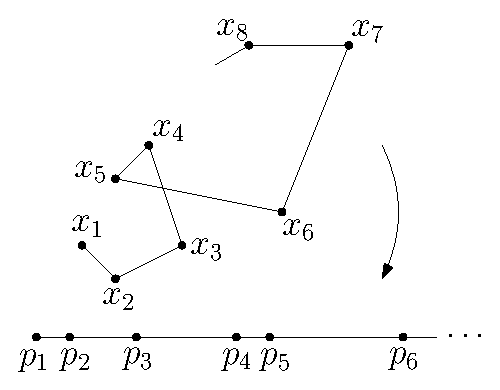
\includegraphics[width=5cm]{figures/decision-path}
    \caption{The Decision Path}
    \label{fig:decisionpath}
\end{figure}

For analytic reasons that become apparent in later sections, we also introduce the \emph{$\delta$-padded decision path} as follows. 
\begin{definition}[$\delta$-padded Decision Path]
Let $\delta = (\delta_t)_{t\in\NN}$ be an increasing sequence of positive numbers and  $p_1, \ldots, p_T$ be a decision path. Then the corresponding $\delta$-padded decision path is the sequence $r_1, \ldots, r_T$ with $r_1 = p_1$ and $r_t = p_t + \delta_t$ for $t>1$.
\end{definition} 

Any online algorithm whose decision space is a subset of Euclidean space, naturally defines a decision path: take $x_t$ to be the decision made at round $t$. For the special case of the OGD algorithm, one has the following lemma for the length of the corresponding decision path. 
\begin{lemma}
  Let $f_t\in C^1_L(\Xcal)$ be convex for all $t\in[T]$ and $(x_t)$ be the sequence of decisions made by OGD. Assume that $(p_t)$ is the decision path for $(x_t)$.
  \begin{enumerate}[label=(\roman*)]
      \item Using step size $\eta_t = \frac{D}{L}t^{-1/2}$, one has for all $t \in [T]$,
         \[ p_t \leq  2D \sqrt{t}. \]
     \item If in addition, $f_t$ are $\alpha$-strongly convex for all $t\in [T]$, then using step size $\eta_t=\frac{1}{\alpha t}$,
         \[ p_t \leq \tfrac{L}{\alpha}(1+\log t). \]
  \end{enumerate}
  \label{lem:ogdpathlength}
\end{lemma}
\begin{proof}
    By the OGD update rule, the Projection Lemma \ref{lem:projection}, and Lipschitz continuity of $f_t$, one gets
 \begin{align*}
   p_{t+1}-p_t &= \|x_{t+1} - x_t\| \\
   &= \|\mathrm{Proj}_\Xcal(x_t - \eta_t\nabla f_t(x_t))-x_t\| \\
  &\leq \|x_t - \eta_t\nabla f_t(x_t)-x_t\| \\
  &= \eta_t\|\nabla f_t(x_t)\| \leq \eta_t L.
 \end{align*}
Since $p_1 = 0$ one can write
\[
  p_t = \sum_{j=1}^{t-1} (p_{j+1} - p_j) \leq L\sum_{j=1}^{t-1} \eta_j.
\]
For (i), we have $\eta_t = \frac{D}{L\sqrt{t}}$ and
   \[
   p_t \leq L\sum_{j=1}^{t-1} \frac{D}{L\sqrt{j}} \leq D \int_0^{t-1} z^{-\frac{1}{2}}\,dz \leq 2D\sqrt{t}.
 \]
% meaning that $r_n \leq (2D + \delta)\sqrt{n}$.
For (ii), we have $\eta_t = \frac{1}{\alpha t}$ and
  \[
    p_t \leq L \sum_{j=1}^{t-1} \frac{1}{\alpha j} \leq \frac{L}{\alpha}(1+\log t). \qedhere
 \]
\end{proof}

\section{Towards No-Regret Consistent Algorithms}\label{sec:towardsolo}

In order to achieve a trade-off between regret and consistency, our algorithm will make use of a basic algorithm $\Acal$, such as OGD, and decide probabilistically at each time step whether to update the current solution point to $\Acal$'s proposal, or to stick to the one from the previous round. Intuitively, we want the updates to be more likely to happen if the current solution point is far away from the $\Acal$'s newly proposed point, but also less likely to happen as the algorithm proceeds and starts converging to a near-optimal solution. As in a Poisson process, the distribution of inter-arrival times is dependent on the \emph{length} of the interval, we will update the algorithm's solution whenever a specific point process on the padded decision path has a hit. 

Concretely, let $\lambda: \RR_+ \to \RR_+$ be an increasing intensity function we will define later. Also define $(r_t)_{t\leq T}$ to be the padded decision path of $\Acal$. We will update the strategy at time $t$ if and only if the non-homogeneous Poisson process with rate $\lambda(\tau)$ had a non-zero count in the interval $(r_{t-1}, r_t].$ This is equivalent to updating with probability  $1 - \exp(-\int_{r_{t-1}}^{r_t} \lambda(\tau)\, d\tau)  = 1 - \exp\{-(M(r_t)- M(r_{t-1}))\}$ (see Lemma~\ref{lem:updatepoisson}). Figure~\ref{fig:poisson} shows an example of the Poisson process and updating procedure.

\begin{figure}[h!]
    \centering
    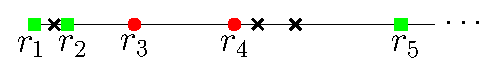
\includegraphics[width=5cm]{figures/poisson}
    \caption{Let $(r_t)$ be the padded decision path. The crosses are the Poisson process events. Red points denote rounds we do not update and green squares are updating rounds. We always update in the first round, and for round $t$, we update only if there is a Poission event on the line segment ending in $r_t$.}
    \label{fig:poisson}
\end{figure}

Observe that this definition satisfies our desiderata from above. Suppose that the algorithm last updated its strategy at time $t' < t$. As the solution drifts, \ie, the distance between $x_{t'}$ and $x_t$ increases, $r_{t'}$ and $r_t$ get further away, and the probability of an update increases. On the other hand, as the gradient steps get smaller (and thus the distance between two consecutive $x$'s decreases), so does the probability of an update. 

We formulate the above in Algorithm~\ref{alg:main_algo}, called Sticky Online Optimization (SOLO). 

\begin{algorithm}[h!] 
    \caption{Sticky OnLine Optimisation (SOLO)}
\label{alg:main_algo}
\begin{algorithmic}
  \STATE $\Acal$ is a no-regret algorithm
  \STATE $\lambda$ an increasing intensity function. 
  \STATE $(\delta_t)$ an increasing padding sequence. 
%  \STATE $\Pi$ is a Poisson process with intensity $\lambda(t)$ 
  \STATE $x_1$ is the first decision proposed by $\Acal$
  \STATE $r_1 \leftarrow 0$
  \STATE $y_1 \leftarrow x_1$ 
  \FOR {$t \in [T]$}
  \STATE Play $y_t$ and receive loss $f_t(y_t)$. 
  \STATE Give $\Acal$ access to the oracle of $f_t$ and set $x_{t+1}$ to be the next proposal of $\Acal$. 
  \STATE $r_{t+1} \leftarrow r_t + \|x_{t+1} - x_t\| + \delta_{t+1} - \delta_t$
  \STATE With probability $1 - \exp\big\{-\big(\int_{r_t}^{r_{t+1}} \lambda(u)\, du\big)\big\}$ \\
  \STATE $\qquad$ Update: set $y_{t+1} \leftarrow x_{t+1}$. 
  \STATE Otherwise set $y_{t+1} \leftarrow y_t$. 
  \ENDFOR
  
%  \FOR{$n \in [N]$}
%\IF{$n = 1$ or $\#(\Pi \cap (r_{n-1},r_n]) \geq 1$}
%      \STATE $y_n\leftarrow x_n$
%    \ELSE
%      \STATE $y_n\leftarrow y_{n-1}$
%    \ENDIF
%    \STATE play $y_n$ and receive loss $f_n(y_n)$
%    \STATE give $\Acal$ access to the oracle of $f_n$, and set $x_{n+1}$ to be the proposal of $\Acal$
%    \STATE $r_{n+1} \leftarrow r_n + \|x_{n+1} - x_n\| + \delta(n+1) - \delta(n)$
%  \ENDFOR
\end{algorithmic}
\end{algorithm}

\section{Analysis of SOLO}
\label{sec:analysis}
The analysis of Algorithm \ref{alg:main_algo} proceeds in two parts. First we relate the regret of SOLO to that of the given algorithm $\Acal$ via a triangle inequality argument, and identify the additional regret paid by Algorithm \ref{alg:main_algo} (Proposition \ref{thm:add-regret}). Then, we prove a technical fact about the distribution of hits in non-homogeneous Poisson processes with sufficiently high intensities (Proposition\ref{lem:bndextraregret}). 

\subsection{Regret}
We analyze the regret of our algorithm as compared to $\Acal$.  Assume that $f_t \in C^1_L(\Xcal)$ for all $t \in [T]$, and let $(x_t)$  be the decisions proposed by $\Acal$, and $(y_t)$ be decisions we actually played. Also denote by $(r_t)$ the padded decision path for $(x_t)$. 

The regret of SOLO is:
\begin{align}
    \Rcal^{\mathrm{SOLO}}(T) &= \sum_{t=1}^T f_t(y_t) - \min_{x^\star\in\Xcal}\sum_{t=1}^T f_t(x^\star) \label{eq:regretbound} \\
    &= \sum_{t=1}^T f_t(y_t) - \sum_{t=1}^T f_t(x_t) 
    +  \sum_{t=1}^T f_t(x_t) - \min_{x^\star\in\Xcal}\sum_{t=1}^T f_t(x^\star) \nonumber \\
    &\leq L\sum_{t=1}^T \|y_t - x_t\| + \Rcal^\Acal(T), \nonumber
  \end{align}
where the last line is due to the Lipschitz continuity of $f_t$ and $\Rcal^\Acal(T)$ is the regret of $\Acal$. Letting $p(t) := \max\{m\leq t: m\text{ is an updating round} \}$ to be the latest updating round before round $t$, it is clear that $y_t = x_{p(t)}$. Using the triangle inequality and remembering that $\delta$ is increasing:
\begin{align*}
  \|y_t - x_t\| &= \|x_t - x_{p(t)}\| \\
  &\leq \sum_{j = p(t)}^{t-1} \|x_{j+1}-x_j\| \\
  &= \sum_{j = p(t)}^{t-1} (r_{j+1} - r_j - [\delta(j+1) - \delta(j)]) \\
    &\leq r_t - r_{p(t)}.
\end{align*}
This gives rise to the definition of \emph{extra regret}: we define the extra regret to be 
\begin{equation}\label{eq:extraregret}
  \Ecal_T = L\cdot\sum_{t=1}^T (r_t - r_{p(t)}).
\end{equation}
The following proposition is now immediate: 
\begin{proposition}
\label{thm:add-regret}
\[
    \Rcal^{\mathrm{SOLO}}(T) \leq  \Ecal_T +\Rcal^\Acal(T).
\]
\end{proposition}
Observe that the extra regret depends directly on the length of the padded decision path. Thus by changing the intensity of the sampling process, we can get a trade-off between the number of changes, and the extra regret. 
%So for having a no-regret algorithm, one requires a sublinear extra regret. Note that in our discussion, the extra regret $\Ecal_N$ along with $\Rcal_N$, $y_n$ and $p(n)$ are random variables and by sublinearity we mean having sublinear expected values.

\subsection{Extra Regret} 
As we saw above, the additional regret of the algorithm depends on the length of the padded decision path between updates. In this section, we present a proposition, bounding this quantity for non-homogeneous Poisson processes with sufficiently fast increasing intensities. 
 
\begin{proposition}\label{lem:bndextraregret}
    Assume $M(\tau) = \omega(\log \tau)$ and $\lambda(\tau) = \omega(1)$ to be increasing. Also assume that $(1/\lambda(\tau))' = o(1)$. Then, for all $t \in [T]$ one has
    \[
        \ev[r_t - r_{p(t)}] \leq C_\lambda/\lambda(r_t),
    \]
    where $C_\lambda$ is a constant only dependent on $\lambda$, and expectation is with respect to the randomness of the Poisson process. Moreover,
    \[
         \ev[\Ecal_T] \leq C_\lambda L\sum_{t=1}^T \frac{1}{\lambda(r_t)}.
    \]
\end{proposition}

At a high level, Proposition~\ref{lem:bndextraregret} implies that we only need to look at the intensity at the last point of the interval (where it is the highest) to bound the expected length of the gap.  

First we bring two supplementary lemmata which are crucial in the proof.
\begin{lemma}\label{lem:suppl1}
  Assuming conditions of Proposition~\ref{lem:bndextraregret}, one has
  \[
    \lim_{\tau\to\infty} \frac{M(\tau)}{\log \int_0^\tau e^{M(u)}\,du} = 1.
  \]
\end{lemma}
\begin{proof}
  Using integration by parts and knowing that $\frac{d}{du}M(u) = \lambda(u)$ we see that
  \[
    \int_0^\tau e^{M(u)}\,du = \tau e^{M(\tau)} - \int_0^\tau u\lambda(u)e^{M(u)}\,du.
  \]
  Now, since the last term is positive, we get
  \begin{align}\label{eq:logupperbnd}
    \log\int_0^\tau e^{M(u)}\,du < \log(\tau e^{M(\tau)}) = M(\tau) + \log \tau.
  \end{align}
  Also, since $\lambda(\tau)$ is increasing, we can write 
  \[
    \int_0^\tau u\lambda(u) e^{M(u)}\,du \leq \tau\lambda(\tau) \int_0^\tau e^{M(u)}\,du,
  \]
  and using the first equality, we arrive at
  \[
    (1 + \tau\lambda(\tau)) \int_0^\tau e^{M(u)}\,du \geq \tau e^{M(\tau)},
  \]
  which gives
  \begin{align}\label{eq:loglowerbnd}
    \log \int_0^\tau e^{M(u)}\,du \geq M(\tau) - \log\frac{1 + \tau\lambda(\tau)}{\tau}.
  \end{align}
  Dividing both sides of \eqref{eq:logupperbnd} by $M(\tau)$ and taking the limsup gives
  \[
    \limsup_{\tau\to\infty} \frac{\log \int_0^\tau e^{M(u)}\,du}{M(\tau)} \leq 1 + \limsup_{\tau\to\infty} \frac{\log \tau}{M(\tau)} = 1, 
  \]
  and doing the same for \eqref{eq:loglowerbnd}, and taking the liminf gives
  \begin{align*}
    \liminf_{\tau\to\infty} \frac{\log \int_0^\tau e^{M(u)}\,du}{M(\tau)} \geq 1 - \limsup_{\tau\to\infty} \frac{\log\frac{1 + \tau\lambda(\tau)}{\tau}}{M(\tau)} \\
    = 1 - \limsup_{\tau\to\infty} \frac{\log\lambda(\tau)}{M(\tau)} = 1, 
  \end{align*}
  since by L'H\^{o}pital's rule the last limit is equal to $1 - \lim_{\tau\to\infty} \frac{\lambda'(\tau)}{\lambda(\tau)^2} = 1$.
  Combining these two inequalities, we can observe that the following limit exists and the equality holds:
  \[
    \lim_{\tau\to\infty} \frac{\log \int_0^\tau e^{M(u)}\,du}{M(\tau)}= 1. \qedhere
  \]
\end{proof}

\begin{lemma}\label{lem:boundingintegral}
  With the same conditions as in Proposition~\ref{lem:bndextraregret}, we have
  \[
      e^{-M(\tau)}\int_0^\tau e^{M(u)}\,du = \Theta(1/\lambda(\tau)) \quad\text{(as $\tau\to\infty$)}
  \]
  Also it also holds that
  \[
    \lim_{\tau\to 0} e^{-M(\tau)}\int_0^\tau e^{M(u)}\,du = 0.
  \]

\end{lemma}
\begin{proof}
 Let us introduce for $\tau > 0$
  \[
    f(\tau) := \log \int_0^\tau e^{M(u)}\,du.
  \]
  Note that the equation in the lemma is equal to $1/f'(\tau)$. Clearly $\lim_{\tau\to\infty} f(\tau) = +\infty$, as well as $\lim_{\tau\to\infty}M(\tau) = +\infty$. So by L'H\^{o}pital's rule and Lemma~\ref{lem:suppl1} above, one gets 
  \[
    \lim_{\tau\to\infty} \frac{M(\tau)}{f(\tau)} = \lim_{\tau\to\infty} \frac{\lambda(\tau)}{f'(\tau)} = 1,
  \]
  which yields
  \[
    \lim_{\tau\to\infty} \frac{ e^{-M(\tau)}\int_0^\tau e^{M(u)}\,du }{1/ \lambda(\tau)} = 1,
  \]
  which is exactly what we wanted.

  For the second argument, observe that as $\tau\to 0$, $e^{-M(\tau)}\to 1$ and $\int_0^\tau e^{M(u)}\,du \to 0$, which completes the proof of this lemma.
\end{proof}

\begin{proof}[Proof of Proposition~\ref{lem:bndextraregret}]
  We begin by deriving the probability distribution of $p(t)$. For all $1 < t \leq T$ and $m \leq t$
  \begin{align*}
      \prob{p(t) = m}  &=\prob{\text{update at } m}\cdot \prob{\text{no updates from $m$ to $t$}}\\
    &= (1 - e^{-(M(r_m) - M(r_{m-1}))})\cdot 
     e^{-(M(r_t) - M(r_m))} \\
     &= e^{-(M(r_t) - M(r_m))} - e^{-(M(r_t) - M(r_{m-1}))}.
  \end{align*}
  Then,
  \begin{align*}
    \ev[r_t - r_{p(t)}] &= \sum_{m=1}^{t-1} (r_t - r_m)(e^{-(M(r_t) - M(r_m))} - e^{-(M(r_t) - M(r_{m-1}))}
) \\
  &= \sum_{m=1}^{t-1}(r_{m+1} - r_{m})e^{-(M(r_t) - M(r_m))} \\
  &= e^{-M(r_{t})}\sum_{m=1}^{t-1}(r_{m+1} - r_{m})e^{M(r_m)} \\
  &\leq e^{-M(r_{t})} \int_0^{r_t} e^{M(u)}\,du.
\end{align*}
Now by Lemma~\ref{lem:boundingintegral}, one gets the desired bound. Also, by linearity of expectation, we get
\begin{equation}\label{eq:extraregretsumbound}
  \ev[\Ecal_T] = L\cdot\sum_{t=1}^T \ev[r_t - r_{p(t)}] \leq C_\lambda L \sum_{t=1}^T \frac{1}{\lambda(r_t)},
\end{equation}
which finishes the proof.
\end{proof}

\section{Online Gradient Descent Trade-offs}\label{sec:ogdtradeoff}
We are now ready to specialize the general algorithm above to obtain our main results. First, we bring a regret-consistency trade-off for OGD for convex and strongly convex functions. Next, we provide trade-offs for online submodular maximisation. We only need to specialize $\delta$ and $\lambda$ to achieve our desired bounds. 

\begin{theorem}[Consistent OGD, I]\label{prop:convex}
  Let $f_t\in C^1_L(\Xcal)$ be convex for all $t\in[T]$. Let $\delta_t = \sqrt{t}$, and denote by $(r_t)$ the padded decision path. For a fixed $\varepsilon\in (0, 1]$  set
  \[
    \lambda(\tau) := (1+\varepsilon)\,\tau^\varepsilon, \quad M(\tau) = \tau^{1 + \varepsilon}.
  \]
  Then,
  \[
      \ev[\kappa_T] = O(T^{\frac{1}{2}+\frac{\varepsilon}{2}}),\quad \ev[\Rcal^{\mathrm{SOLO}}(T)] = O(T^{1-\frac{\varepsilon}{2}}).
  \]
\end{theorem}
\begin{proof}
  It is easy to check that $\lambda(\tau)$ and $M(\tau)$ satisfy the conditions of Proposition~\ref{lem:bndextraregret}. Therefore,
  \[
    \ev[r_t - r_{p(t)}] \leq \frac{C_\lambda}{\lambda(r_t)} \leq \frac{C_\lambda}{\lambda(\sqrt{t})} = \frac{C_\lambda}{(1+\varepsilon)}t^{-{\frac{\varepsilon}{2}}}.
  \]
  Then,
  \[
      \ev[\Ecal_T] \leq \frac{C_\lambda L}{(1+\varepsilon)}\sum_{t=1}^T t^{-{\frac{\varepsilon}{2}}} \leq \frac{C_\lambda L}{(1+\varepsilon)(1-\frac{\varepsilon}{2})} T^{1 - \frac{\varepsilon}{2}} = O(T^{1 - \frac{\varepsilon}{2}}).
  \]
  By Theorem~\ref{thm:ogd}, we know that $\Rcal_\Acal(T) = O(\sqrt{T})$. Hence 
  \[
      \ev[\Rcal^{\mathrm{SOLO}}(T)] = O(T^{1 - \frac{\varepsilon}{2}}).
  \]

  Finally, to bound $\kappa_T$, recall that the total path length from  Lemma~\ref{lem:ogdpathlength} (i), and the final padding of $\delta(T) = \sqrt{T}$.  Since $M(\tau)$ is increasing, we get
  \begin{align}\label{eq:ogdkappabound}
    \ev[\kappa_T] \leq M(r_T) \leq M((2D + 1)\sqrt{T}) \nonumber \\ = (2D + 1)^{1+\varepsilon}T^{\frac{1}{2}+\frac{\varepsilon}{2}} = O(T^{\frac{1}{2}+\frac{\varepsilon}{2}}),
  \end{align}
  where the first inequality is due to the fact that the number of Poisson points is always greater than the number of rounds that we update.
\end{proof} 

We can use a similar analysis in the strongly convex case. 
\begin{theorem}[Consistent OGD, Strongly Convex Functions]\label{prop:sconvex}
  Let $f_t\in C^1_L(\Xcal)$ be $\alpha$-strongly convex, for all $t\in[T]$. Let $\delta_t = \log t$, and denote by $(r_t)$ the padded decision path. Finally, let $\gamma := 1 + \frac{L}{\alpha}$. For a fixed $\varepsilon\in(0,1)$ set:  
  \[
    \lambda(\tau) := \exp\rbr{\varepsilon\tfrac{\tau}{\gamma}}, \quad M(\tau) = \frac{\gamma}{\varepsilon}(\exp\rbr{\varepsilon\tfrac{\tau}{\gamma}}-1).
  \]
  Then one has
  \[
      \ev[\kappa_T] = O(T^{\varepsilon}),\quad \ev[\Rcal^{\mathrm{SOLO}}(T)] = O(T^{1-\varepsilon\frac{1}{\gamma}}).
  \]
\end{theorem}
\begin{proof}
  By Lemma~\ref{lem:ogdpathlength} and the choice of $\delta_\cdot$,  since $M(\tau)$ is increasing: 
  \begin{equation}\label{eq:scogdkappabound}
    \ev[\kappa_T] \leq M(r_T) \leq M(\gamma(1+\log T)) = O(T^{\varepsilon}).
  \end{equation}
  Also, by Proposition~\ref{lem:bndextraregret} and integral approximation we get
  \begin{equation}
    \ev[\Ecal_T] \leq C + C\int_1^T \frac{1}{\lambda( \log u)}\,du = O(T^{1-\varepsilon\frac{1}{\gamma}}). \qedhere
  \end{equation}
\end{proof}

\begin{remark}\label{rem:lengthasymp}
    The reader should be convinced by now that for any online algorithm that has well-behaved asymptotic decision path length, one can use the SOLO algorithm using the right intensity function $\lambda$, and get a consistency/regret trade-off. Thus, a key element in using SOLO as an add-on to an online algorithm is to analyse the decision path length's asymptotics.
\end{remark}

To further show the extent of freedom in choosing $\lambda$, we bring another theorem on another type of trade-off for standard OGD.
\begin{theorem}[Consistent OGD, II]
   Let $f_t\in C^1_L(\Xcal)$ be convex for all $t\in[T]$. Let $\delta_t = \sqrt{t}$, and denote by $(r_t)$ the padded decision path. Set
  \[
      \lambda(\tau) := \log(1+\tau) + \frac{\tau}{1+\tau}, \quad M(\tau) = \tau\log(1 + \tau).
  \]
  Then,
  \[
      \ev[\kappa_T] = \tilde{O}(\sqrt{T}),\quad \ev[\Rcal^{\mathrm{SOLO}}(T)] = O(T/\sqrt{\log T}) = o(T).
  \]
\end{theorem}
\begin{proof}
    It is easy to verify that $\lambda$ and $M$ satisfy the conditions of Proposition~\ref{lem:bndextraregret}.  Following the same line of proof as Theorem~\ref{prop:convex}, we arrive at 
    \[
        \ev[\Ecal_T] \leq C_\lambda\sum_{t=1}^T \frac{1}{\lambda(\sqrt{t})} \leq C_\lambda\int_1^T \frac{du}{\lambda(\sqrt{u})} = C_\lambda \int_1^T \frac{du}{\log(1+ \sqrt{u}) + \frac{\sqrt{u}}{1+\sqrt{u}}}.
    \]
    By a change of variable $v = \sqrt{u}$, we see the last integral is equal to
    \[
        \int_1^{\sqrt{T}} \frac{2v\,dv}{\log(1+v) + \frac{v}{1+v}} = 
        \int_1^{\sqrt{T}} \frac{2\,dv}{\frac{\log(1+v)}{v} + \frac{1}{1+v}}.
    \]
    By Harmonic Mean-Geometric Mean inequality, we obtain
    \[
        \leq  \int_1^{\sqrt{T}} \sqrt{\frac{v(1+v)}{\log(1+v)}}\,dv < \int_1^{\sqrt{T}} \frac{1+v}{\sqrt{\log(1+v)}}\,dv.
    \]
    But one can show that the following asymptotics hold:
    \[
        \int \frac{\tau}{\sqrt{\log \tau}}\,d\tau = \sqrt{\frac{\pi}{2}}\cdot\mathrm{erfi}(\sqrt{2\log \tau}) = O\left(\frac{\tau^2}{\sqrt{\log \tau}}\right),
    \]
    resulting in
    \[
        \ev[\Ecal_T] = O\left(\frac{T}{\sqrt{\log T}}\right).
    \]

    For proving the bound on $\kappa_T$, we need to evaluate 
    \[
        \ev[\kappa_T] \leq M(r_T) \leq M((2D + 1)\sqrt{T}) = O(\sqrt{T}\log T) = \tilde{O}(\sqrt{T}). \qedhere
    \]
\end{proof}

One can also show that, given our analysis, the results above are optimal. This is explained for OGD (Theorem~\ref{prop:convex}) below. Thus, better results cannot be obtained by changing $\lambda$, if we keep the analysis untouched.
\begin{theorem}[OGD Optimality]\label{thm:optimality} Let $\lambda$ be an intensity function that satisfies the conditions of Proposition~\ref{lem:bndextraregret}. Assuming the same analysis and using integral approximations, SOLO on top of OGD results in an  algorithm which satisfies
    \[
        \widehat{\kappa_T}\cdot \widehat{\Ecal_T} = \Omega(T^{3/2}),
    \]
    where $\widehat{\kappa_T}$ and $\widehat{\Ecal_T}$ are estimates (upper bounds) used in analysis of SOLO for their respective expectations.
\end{theorem}
\begin{proof}
    Recall that in the proof of bounding the extra regret $\Ecal_T$ in Theorem~\ref{prop:convex}, we arrived to the upper bound
    \[
        \ev[\Ecal_T] \leq C_\lambda \int_1^T \frac{du}{\lambda(\sqrt{u})} = C_\lambda \int_1^{\sqrt{T}} \frac{2u\,du}{\lambda(u)} =: \widehat{\Ecal_T},
    \]
    for which we proved in the case $\lambda(\tau) = (1+\varepsilon)\tau^\varepsilon$ to be of $O(T^{1- \frac{\varepsilon}{2}})$. We keep the integral as our estimate for $\ev[\Ecal_T]$. For consistency cost, the upper bound
    \[
        \ev[\kappa_T] \leq  M((2D+1)\sqrt{T}) = \int_0^{(2D + 1)\sqrt{T}} \lambda(u)\,du =: \widehat{\kappa_T}
    \]
    is available. By Cauchy-Schwartz inequality in $L^2$ we have
    \[
        \widehat{\kappa_T}\cdot \widehat{\Ecal_T} \geq C\cdot\left( \int_1^{\sqrt{T}} \frac{u\, du}{\lambda(u)} \right) \left( \int_1^{\sqrt{T}} \lambda(u)\,du \right) \geq C \left(\int_1^{\sqrt{T}} \sqrt{u}\,du \right)^2 =\frac{4C}{9}(T^{3/4} - 1)^2 = \Omega(T^{3/2}).\qedhere
    \]
\end{proof}
\section{Online Submodular Maximisation Trade-offs}\label{sec:submodapplication}
In this section we show that a similar set of ideas apply to the problem of online submodular function maximisation. Note that in this case, due to hardness (see Theorem~\ref{thm:hardnesssubmod}), our goal is to find trade-offs between approximate $\beta$-regret and consistency for different classes of submodular functions. We give examples for two special cases: monotone DR-submodular functions~\cite{bian2016guaranteed} and monotone submodular set functions~\cite{nemhauser1978analysis}. 

 
By selectively deciding when to update the solution, we transform it to an algorithm that suffers an extra regret of $O(T^{1-\frac{\varepsilon}{2}})$ in expectation, while updating at most $O(T^{\frac{\varepsilon + 1}{2}})$ times.

We further extend the analysis to the discrete case, where the utility functions are submodular set functions and the optimisation domain is a matroid $\Mcal$. Using the Swap-Rounding technique (see Section~\ref{sec:rounding}) to round the solutions of online gradient ascent algorithm, we get an algorithm  that achieves sublinear $\frac{1}{2}$-regret. We can then be selective on when to apply the updates to achieve additional additive regret of $T^{1 - \frac{\varepsilon}{2}}$ using at most $O(T^{\frac{\varepsilon + 1}{2}})$ updates. 


\subsection*{DR-Submodular Case} 
We can use our result to devise a consistent online DR-submodular maximisation algorithm, using the simple fact that our regret analysis is additive with respect to $\Ecal_t$. Namely, if we add $\sum_{t=1}^T f_t(x_t) - \sum_{t=1}^T f_t(y_t)$ to \eqref{eq:halfreg-dr-subm}, we get the notion of $\frac{1}{2}$-regret for the sequence $(y_t)$. The rest of the analysis follows immediately: by being consistent, one suffers an extra regret of $O(T^{1-\frac{\varepsilon}{2}})$ in expectation, while updating at most $O(T^{\frac{\varepsilon + 1}{2}})$ times.

\subsection*{Monotone Submodular Case} We now relate the DR-Submodular result to the discrete case, where the utility functions are submodular set functions and the optimisation domain is a matroid $\Mcal$. 

Taking the online stochastic setting, we assume that in each round, the player can evaluate the multilinear extension of the submodular utility, as well as its gradients. With a few modifications of the consistent OGD algorithm, one can design an algorithm for this discrete case, as described in Algorithm~\ref{alg:submod_algo}.

\begin{algorithm}[ht] 
\caption{Consistent Online Submodular Maximization}
\label{alg:submod_algo}
\begin{algorithmic}
    \STATE $x_1 \leftarrow$ a point in $\Xcal = \Pcal(\Mcal)$.
  \STATE $S_1 \leftarrow$ rounded set of $x_1$.
  \STATE $r_1 \leftarrow 0$.

  \FOR {$t \in [T]$}
  \STATE Play $S_t$ and receive loss $f_t(S_t)$. 
  \STATE $x_{t+1} \leftarrow \mathrm{Proj}_\Xcal(x_t + \eta_t \nabla F_t(x_t))$
  \STATE $r_{t+1} \leftarrow r_t + \|x_{t+1} - x_t\| + \sqrt{t+1} - \sqrt{t}$
  \STATE With probability $1 - \exp(-(r_{t+1}^{1+\varepsilon}- r_{t}^{1+\varepsilon}))$
  \STATE $\qquad$ Update: set $S_{t+1} \leftarrow \mathrm{round}_\Mcal(x_t)$.
  \STATE Otherwise set $S_{t+1} \leftarrow S_t$.
  \ENDFOR
\end{algorithmic}
\end{algorithm}

It is clear that the same bounds for consistency cost in the case of DR-submodular functions holds for this algorithm as well (note that the multilinear extension is DR-submodular, see Lemma~\ref{lem:multiproperties}). To provide the regret bounds, we first take the expectation w.r.t. the distribution induced by rounding, and then, w.r.t. the probability of updating. By the property of Swap-Rounding (Theorem~\ref{thm:swaprounding}), for any sequence $y_1, \ldots, y_T \in \Xcal$ we have
\[
    \ev_{S_t}[f_t(S_t)] \geq F_t(y_t)
\]
Also, since sum of submodular functions is submodular and the multilinear extension is an extension, we have
\[
    \max_{x^\star\in \Xcal} \sum_{t=1}^T F_t(x^\star) \geq \max_{S^\star\in \Mcal} \sum_{t=1}^T f_t(S^\star).
\]
Therefore, by summing the inequalities we can get
\begin{align*}
    \frac{1}{2}\max_{x^\star\in \Xcal} \sum_{t=1}^T F_t(x^\star) - \sum_{t=1}^T F_t(y_t) \geq \ev\left\{ \frac{1}{2}\max_{S^\star\in \Mcal} \sum_{t=1}^T f_t(S^\star) - \sum_{t=1}^T f_t(S_t) \right\},
\end{align*}
which means that the expected value of $\frac{1}{2}$-regret for the discrete setting is upper bounded by the $\frac{1}{2}$-regret of the DR-submodular setting. Taking expectation w.r.t. the probabilities of updates, gives the desired result.

\begin{remark}
    Note that we did not use the fact that the initial online algorithm is no $\frac{1}{2}$-regret. If the initial algorithm is in general a no $\beta$-regret algorithm with a decision path length of $O(\sqrt{T})$, one gets the same result.
\end{remark} 



\chapter{Regularisation}\label{chap:rftl}
In the previous chapter, we came up with a meta-algorithm that can be used for two types of OGD, as well as (discrete and continuous) online submodular maximisation. The only requirement of our meta-algorithm is a well-behavied decision path length asymptotics, as well as Lipschitz-continuity of loss (or utility) functions. In this chapter, we go a step further and show that our meta-algorithm can be used for the large class of regularised online algorithms. Concretely, we will show that for these online algorithms the behaviour of the decision path length can be controlled, and derive consistency/regret trade-offs.

\section{Basic Notions}
\subsubsection*{Dual Spaces and Dual Norms}
Let $E$ be a finite dimensional normed vector space over $\RR$, with norm $\|\cdot\|$. The \emph{dual space} $E^\star$ is defined as the space of all linear functionals over $E$, that is,
\[
    E^\star = \{ l\from E\to \RR \mid l\text{ is linear} \}.
\]
One knows from linear algebra that $E^\star$ is a vector space with the same dimension as $E$. 
For $v\in E$ and $l\in E^\star$, the value $l(v)$ is also denoted by $\inner{l}{v}$ (not to be confused with an inner product).\footnote{Indeed, if $E$ is an inner product space, and the norm is defined via the inner product, by Riesz representation theorem, one can identify $l$ with a vector $u\in E$ and $l(v) = \inner{u}{v}$ is actually the inner product of $u$ and $v$.} Moreover, one can equip $E^\star$ with a norm, defined as
\[
    \|l\|^\star = \max_{\|x\| = 1} |\inner{l}{x}|.
\]

\subsubsection*{Fenchel Conjugates}
Let $\phi\from E \to \RR$ be a differentiable strictly convex function. One can associate a function $\phi^\star\from E^\star \to \RR$ called the \emph{Fenchel conjugate} of $\phi$, defined as
\[
    \phi^\star (l) = \sup_{x\in E} \{ \inner{l}{x} - \phi(x) \}. 
\]

Of particular interest is the Fenchel conjugate of a quadratic function $\phi(x) = \frac{1}{2}\inner{Ax}{x}$ for a symmetric positive definite matrix. One can compute $\phi^\star(l) = \frac{1}{2}\inner{A^{-1}l}{l}$. 

One of our uses of Fenchel duality is the following lemma, which explains the relation between a strongly convex function and its dual. Before proceeding, we remind the reader of the notion of a \emph{smooth} convex function.
\begin{definition}[Smooth Convex Function]
    A $C^1$ function $f \from E\to \RR$ is $\beta$-smooth with respect to the norm $\|\cdot\|$, if for all $x,y\in E$,
    \[
        f(y) \leq f(x) + \inner{\grad f(x)}{y-x} + \frac{\beta}{2}\|x-y\|^2.
    \]
\end{definition}
\begin{lemma}[{Strong/Smooth Duality}] \label{lem:strongsmoothdual}
    Suppose that $\phi \from E\to \RR$ is a closed and convex function. Then $\phi$ is $\alpha$-strongly convex with respect to a norm $\|\cdot\|$ if and only if $\phi^\star$ is $\frac{1}{\alpha}$-strongly smooth with respect to the dual norm $\|\cdot\|^\star$.
\end{lemma}
A proof of this lemma can be found in \citet{zalinescu2002convex}. Moreover, the relation between the Hessian of a function and its conjugate is described by the following theorem, which we bring a simplified reformulation here.
\begin{theorem}[{\citet[Theorem 2.4]{rockafellar1990generalized}}]\label{thm:rock}
    The function $f$ is twice differentiable at $x$ relative to the vector $v = \grad f(x)$ if and only if its conjugate $f^\star$ is twice differentiable at $v$ relative to the vector $x = \grad f^\star(v)$. Then the functions
    $\frac{1}{2} D^2 f(x)$ and $\frac{1}{2} D^2 f^\star(x)$  are conjugate to each other.
\end{theorem}

\subsubsection*{Matrix and Local Norms}
Let $A$ be a positive semi-definite matrix. One can introduce a \emph{matrix norm} on $E$ based on $A$ as
\[
    \|x\|_A = \sqrt{\inner{Ax}{x}}.
\]
It can be shown that the dual norm to this matrix norm is a matrix norm defined via $A^{-1}$, that is, $\|x\|_{A}^\star = \|x\|_{A^{-1}}$.

For a twice differentiable map $\phi\from E \to \RR$ which admits a Hessian, one can define a matrix norm at each point $z\in E$ as
\[
    \|x\|_z := \|x\|_{D^2\phi(z)} = \sqrt{\inner{D^2\phi(z)(x)}{x}},
\]
which we refer to as the \emph{local norm} at $z$.

\section{Consistent Regularised Follow the Leader}
In this section we bring the Regularised Follow The Leader (RFTL) algorithm, and describe its main properties which are related to this thesis. The reader is referred to \citet{hazan2016introduction} for further details. We then provide asymptotics for the decision path length of RFTL, resulting in a consistency/regret trade-off.

As before, the decision space $\Xcal$ is assumed to be a convex and compact subset of $E$. Let $\phi\from E \to \RR$ be a strongly convex and smooth regulariser, that in the interior of $\Xcal$ has a Hessian.

\begin{algorithm}[h!] 
    \caption{Regularised Follow The Leader}
\label{alg:rftl_algo}
\begin{algorithmic}
    \STATE $\phi$ is a regularisation function.
    \STATE $\Xcal$ is a compact convex set in $E$.
    \STATE $\eta$ is the step size.
    \STATE $x_1 \leftarrow \argmin_{x \in \Xcal} \phi(x)$ is the first decision.
    \FOR {$t \in [T]$}
    \STATE Play $x_t$ and receive loss $f_t(x_t)$ and the gradient $\grad_t := \grad f_t(x_t)$.
    \STATE Update
    \[
        x_{t+1} = \argmin_{x\in \Xcal} \left\{ \eta \sum_{s=1}^{t} \inner{\nabla_s}{x} + \phi(x) \right\}
    \]
    \ENDFOR
\end{algorithmic}
\end{algorithm}

\begin{theorem}[{\citet[Theorem 5.1]{hazan2016introduction}}]\label{thm:rftl}
    For every $u \in \Xcal$, Algorithm~\ref{alg:rftl_algo} attains the following bound on regret:
    \[
        \Rcal(T) \leq 2\eta \sum_{t=1}^T\|\grad_t\|_t^{\star 2} + \frac{1}{\eta}(\phi(u) - \phi(x_1)).
    \]
    Moreover, if for all $t\in[T]$ the gradients satisfy $\|\grad_t\|_t^{\star} \leq G_\phi$, by optimising $\eta$, one gets
    \[
        \Rcal(T) \leq 2D_\phi G_\phi \sqrt{2T},
    \]
    where $D_\phi$ is the \emph{diameter} of $\Xcal$ with respect to $\phi$, defined as
    \[
    D_\phi = \sqrt{\max_{x,y\in\Xcal} \{\phi(x) - \phi(y)\} }.
    \]

\end{theorem}

We do not bring the proof here, but we explain some of the important machinery used in the proof, the first of which is the notion of a Bregman divergence.

\begin{definition}[Bregman Divergence]
    Let $\phi\from E \to \RR$ be strongly convex and $C^1$. The Bregman divergence between two points $x,y\in E$ with respect to $\phi$ is defined as
    \[
        B_\phi(x, y) := \phi(x) - \phi(y) - \inner{\grad\phi(y)}{x-y}.
    \]
\end{definition}

Note that if $\phi$ is twice differentiable, by the Mean Value Theorem one knows that the second order Taylor approximation is exact if one computes the Hessian at an intermediate point, \ie, 
\[
    B_\phi(x, y) = \frac{1}{2}\inner{D^2\phi(z)(x-y)}{ x-y},
\]
for some $z \in [x, y]$. With the language of local norms, this can be written as
\begin{equation}\label{eq:defnlocalnorm}
    B_\phi(x, y) = \frac{1}{2}\|x-y\|_z^2.
\end{equation}
In situations where $z$ is not used, we just write $\|\cdot\|_{x,y}$. A special local norm which is used in the proof and our analysis is the local norm at round $t$ of RFTL, that is, the one relating to Bregman divergence between $x_t$ and $x_{t+1}$. We denote this norm by
\[
    \|\cdot \|_t := \|\cdot\|_{x_t, x_{t+1}}.
\]



\begin{lemma}
    Let $x_t$ and $x_{t+1}$ be two consecutive decisions made by RFTL. Also let $\grad_t\in E^\star$ to be the gradient of $f_t$ at the point $x_t$. Then, it holds
    \[
        \|x_t - x_{t+1}\|_t \leq 2\eta\cdot \|\grad_t\|_t^\star. 
    \]
\end{lemma}
\begin{proof}
    This prove follows Hazan's. Define for $t\in[T]$ the function $F_t$ as
    \[
        F_t(x) = \eta \sum_{s=1}^{t} \inner{\nabla_s}{x} + \phi(x).
    \]
    The Taylor approximation at $x_{t+1}$ gives
    \begin{align*}
        F_t(x_t) &= F_t(x_{t+1}) + \inner{\grad F_t(x_{t+1})}{x_t - x_{t+1}} + B_{F_t}(x_t, x_{t+1}) \\
                 &\geq F_t(x_{t+1}) +  B_{F_t}(x_t, x_{t+1}) \quad\quad  \text{($x_{t+1}$ is a minimiser of $F_t$ over $\Xcal$)} \\
                 &= F_t(x_{t+1}) +  B_\phi(x_t, x_{t+1}),
    \end{align*}
    where the last line is due to the fact that linear terms do not affect the Bregman divergence. Hence,
    \begin{align*}
        B_\phi(x_t, x_{t+1}) &\leq F_t(x_t) - F_t(x_{t+1}) \\
                             &= F_{t-1}(x_t) - F_{t-1}(x_{t+1}) + \eta\inner{\grad_t}{x_t - x_{t+1}} \\
                             &\leq \eta\inner{\grad_t}{x_t - x_{t+1}},
    \end{align*}
    as $x_t$ is the minimiser of $F_{t-1}$ over $\Xcal$. By \eqref{eq:defnlocalnorm} and the Cauchy-Schwarz inequality, one gets
    \begin{align*}
        \frac{1}{2}\|x_t - x_{t+1}\|_t^2 = B_\phi(x_t, x_{t+1}) \leq  \eta\inner{\grad_t}{x_t - x_{t+1}} \leq \eta\cdot \|\grad_t\|_t^\star \cdot \|x_t - x_{t+1}\|_t.
    \end{align*}
    Hence, the lemma follows.
\end{proof}

 Our main goal in the rest of this section is to give a bound on decision path length.

\begin{lemma}
    Let $x_t$ and $x_{t+1}$ be two consecutive decisions made by RFTL. Also, let $\grad_t$ be the gradient of $f_t$ at round $t$. Then
    \[
        \|x_t - x_{t+1}\|_t \geq \sqrt{\alpha} \cdot \|x_t - x_{t+1}\|,
    \]
    and
     \[
         \|\grad_t\|_t^\star \leq \frac{1}{\sqrt{\alpha}}\cdot \|\nabla_t\|^\star.
     \]
\end{lemma}
\begin{proof}
    By definition of local norm, equation \eqref{eq:defnlocalnorm}, and strong convexity, one has
    \begin{align*}
        \frac{1}{2}\|x_t - x_{t+1}\|_t^2 &= B_\phi(x_t, x_{t+1})\\
                                         &= \frac{1}{2}\inner{D^2\phi(z)(x_t-x_{t+1})}{x_t-x_{t+1}} \\
                                         &\geq \frac{\alpha}{2} \|x_t-x_{t+1}\|^2,
    \end{align*}
    thus, the first inequality follows. For the second inequality, we observe that by Lemma~\ref{lem:strongsmoothdual}, $\phi^\star$ is $1/\alpha$-smooth, and by using Theorem~\ref{thm:rock}, we get
    \begin{align*}
        \|\grad_t\|_t^{\star 2} = \inner{  D^{-2}\phi(z)\grad_t } {\grad_t} = \inner{  D^2\phi^\star(z)\grad_t } {\grad_t} \leq \frac{1}{\alpha} \|\grad_t\|^{\star 2}, 
    \end{align*}
    and the inequality follows.
\end{proof}
\begin{corollary}\label{cor:lenstep}
    One has
    \[
        \|x_t - x_{t+1}\| \leq 2\cdot\frac{\eta}{\alpha}\cdot \|\grad_t\|^\star.
    \]
    Moreover, if $f_t$ are $L$-Lipschitz with respect to the norm $\|\cdot\|$ for all $t\in[T]$, by choosing $\eta = \frac{D_\phi}{L} \sqrt{\alpha/2T}$ one gets the optimal regret bound for RFTL, and 
    \[
        \|x_t - x_{t+1}\| \leq \frac{2\eta}{\alpha}L = D_\phi \sqrt{\frac{2}{\alpha T}}.
    \]
\end{corollary}

The careful reader may have noticed that the step size $\eta$ is fixed in the analysis above, and is dependent on $T$, that is, the asymptotics we get for the length of the decision path will be linear, which does not let us to use our consistent meta-algorithm on top of RFTL. However, using a trick called the ``Doubling Trick'' we can overcome this situation, and regularly decrease $\eta$ over time. The trick is explained in the following lemma.

\begin{lemma}[{Doubling Trick, \citet[Section 2.3.1]{shalev2012online}}]
    Consider an algorithm $\Acal$ that enjoys a regret bound of the form $C\sqrt{T}$, but its parameters (such as $\eta$) require the knowledge of $T$. By running $\Acal$ on the $2^m$ rounds $t = 2^m,\ldots,2^{m+1} -1$ for $m\in \NN$, $\Acal$ does not need to know the time horizon, and the regret of this new algorithm is at most $\frac{\sqrt{2}}{\sqrt{2} - 1}C\sqrt{T}$.
\end{lemma}

It follows from the lemma above and Theorem~\ref{thm:rftl}, that using the Doubling Trick, we can assume that 
\[
    \frac{D_\phi}{L} \sqrt{\alpha/2}\cdot t^{-1/2} \leq \eta_t \leq \frac{D_\phi}{L} \sqrt{\alpha} \cdot t^{-1/2}.
\]
Moreover, from Corollary~\ref{cor:lenstep} it follows that 
\[
    \|x_t - x_{t+1}\| \leq  2D_\phi \sqrt{\frac{1}{\alpha t}}.
\]
Hence, the decision path length is of $O(\sqrt{T})$. By the same analysis as for Consistent OGD (Theorem~\ref{prop:convex}), we get the following trade-off.
\begin{theorem}[Consistent RFTL]
    Using the same Poisson process intensity as of Consistent OGD, one has the following trade-off for Consistent RFTL, for every $\varepsilon \in [0, 1)$:
   \[
      \ev[\kappa_T] = O(T^{\frac{1}{2}+\frac{\varepsilon}{2}}),\quad \ev[\Rcal^{\mathrm{SOLO}}(T)] = O(T^{1-\frac{\varepsilon}{2}}).
   \]
 
\end{theorem}

%\section{Example: Experts Advice}\label{sec:experts}
%\textbf{TODO: bring up the experts problem\dots}
%This result, however, is sub-optimal, as compared to \citet{altschuler2018online}.


\chapter{Experimental Results}

\begin{figure*}[pt]
    \centering
    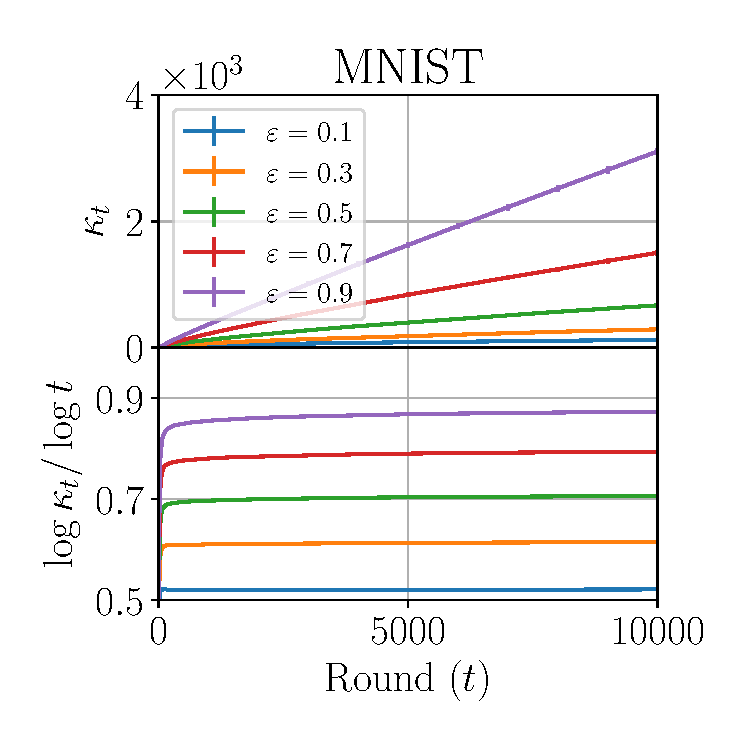
\includegraphics[width=.45\textwidth]{figures/mnist-consistency}%
    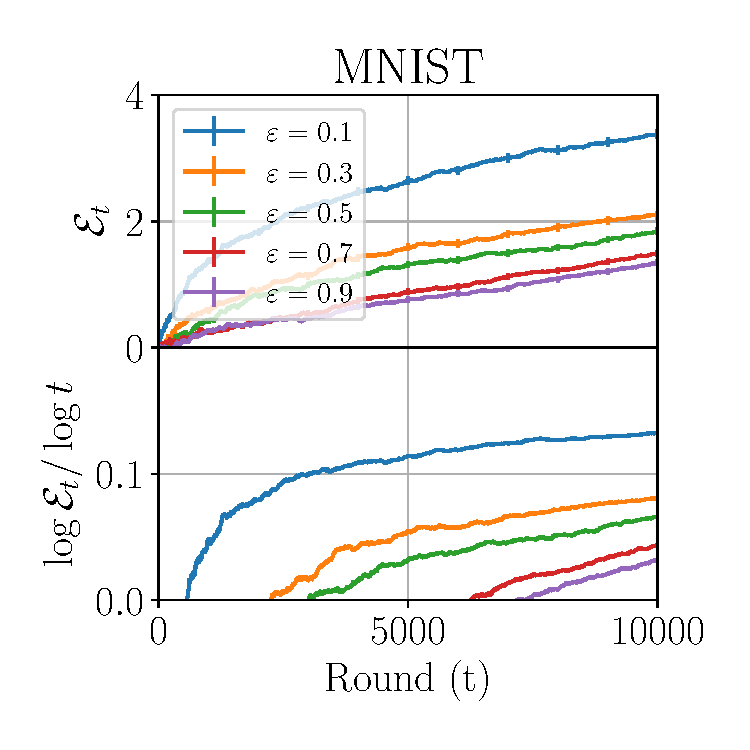
\includegraphics[width=.45\textwidth]{figures/mnist-extra-regret}\\
    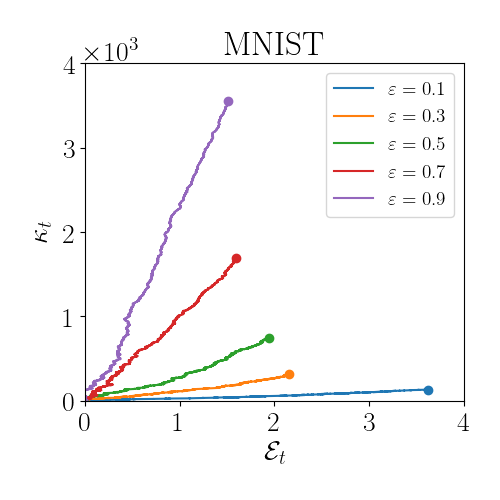
\includegraphics[width=.45\textwidth]{figures/mnist-extra-reg-vs-consistency}%
    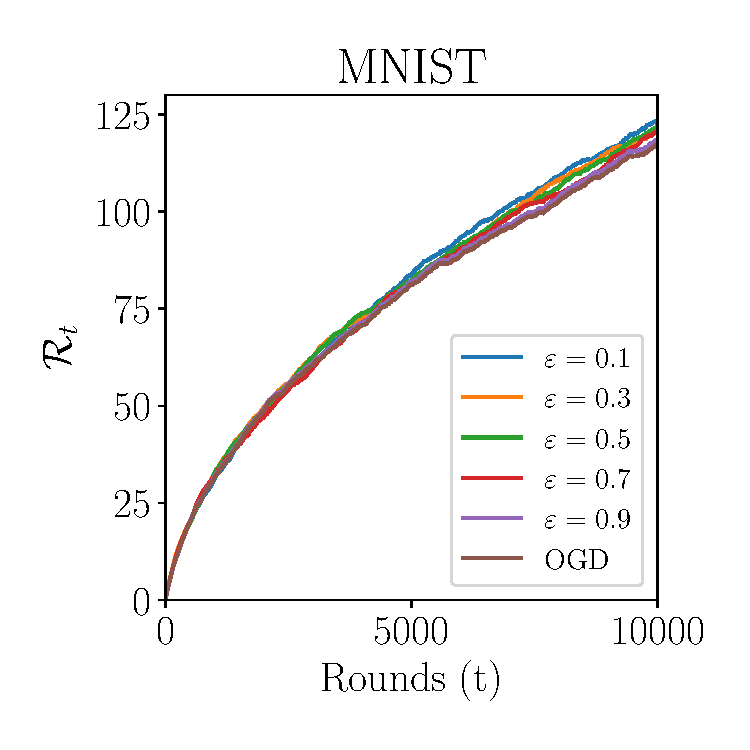
\includegraphics[width=.45\textwidth]{figures/mnist-regret}
     \caption{Experimental results for Online Convex Optimisation on MNIST dataset.}
    \label{fig:experiments1}
\end{figure*}
\begin{figure*}[pt]
    \centering
    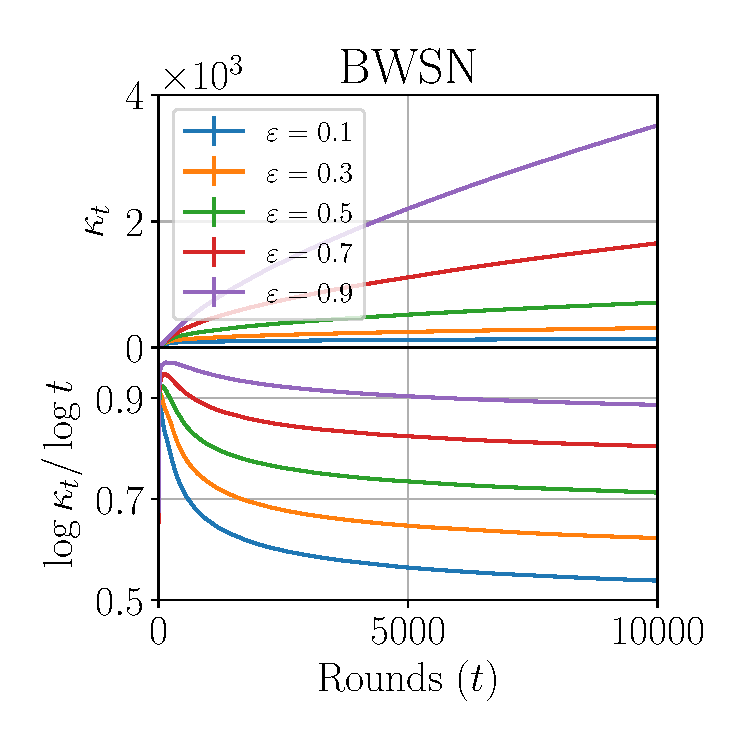
\includegraphics[width=.45\textwidth]{figures/bwsn-consistency}%
    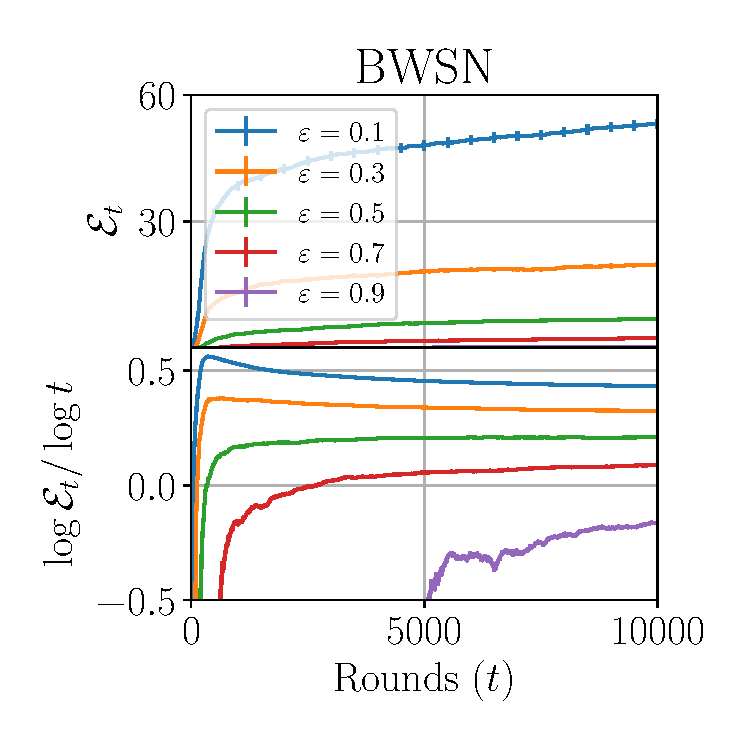
\includegraphics[width=.45\textwidth]{figures/bwsn-extra-regret}\\
    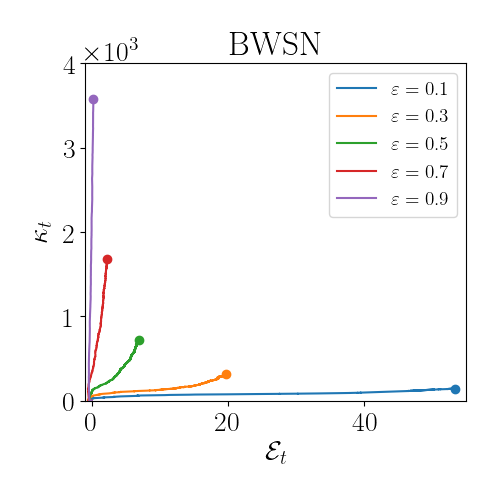
\includegraphics[width=.45\textwidth]{figures/bwsn-extra-reg-vs-consistency}%
    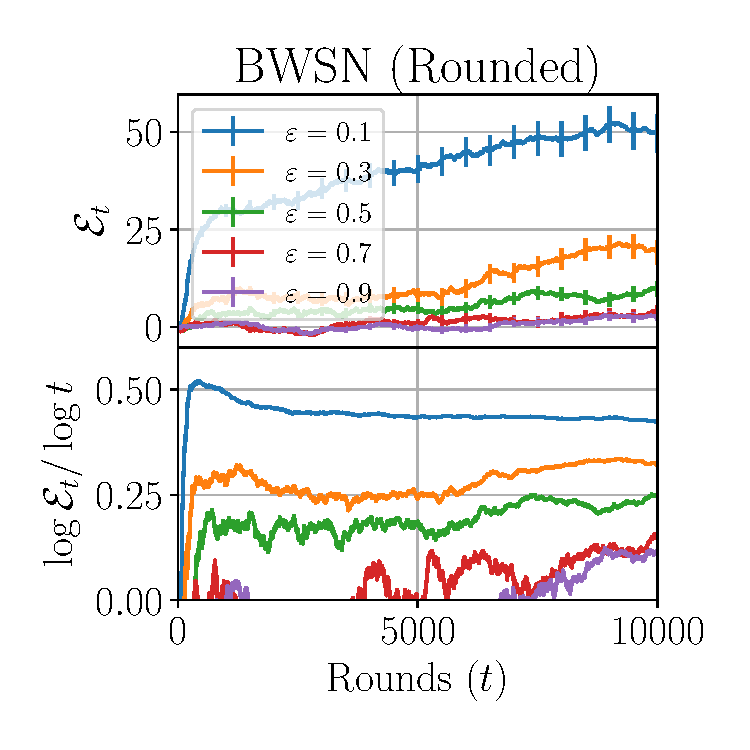
\includegraphics[width=.45\textwidth]{figures/bwsn-extra-regret-rounded}
    \caption{Experimental results for Online Submodular Maximisation for the BWSN problem.}
    \label{fig:experiments2}
\end{figure*}

We evaluate the performance of our algorithm for different parameters of $\varepsilon$, demonstrating different points on the consistency vs. regret trade-off curve. Overall, we find that while the base algorithm $\mathcal{A}$ updates the solution at every time step, overwhelmingly we suffer very little additional regret when we choose to update significantly fewer times. 

\section{Experiments}
We focus on two cases: Online Convex Optimisation and Online Submodular Maximisation.
\subsection*{Online Convex Optimisation} We perform Online Logistic Regression on the MNIST dataset of handwritten digits \citep{lecun1998mnist}, to distinguish digit 3 from 5 over the unit $\ell_1$ ball. The training data consists of 11\,552 images labeled with either $1$ or $-1$, and at each round, an image $u$ is selected uniformly at random. The algorithm proposes a vector $w$, and the incurred loss would be
\[
    f(w) = \log(1 + e^{-y\cdot(u^\top w)}),
\]
where $y$ is the label for the image. In this setting, the expected regret is defined as:
\[
    \mathcal{R}_T = \sum_{t=1}^T f_t(x_t) - T\cdot\min_{\|x\|_1 \leq 1} \ev[f(x)],
\]
where the expectation is evaluated over the training set.

\subsection*{Online Submodular Maximisation}
We investigate the problem introduced in the Battle of the Water Sensor Networks challenge \citep{ostfeld08bwsn}, where the goal is to find the best set of sensor locations to detect a contamination event, minimising detection time.

In our experiment, we select 20 sensors from among 12\,527 possible locations, based on performance on a set of contamination events.  As \citet{leskovec07cost} showed, this problem can be formulated as an instance of the facility location problem: For any subset of sensor locations $S$, every contamination event is a submodular function $f_e(S) := \max_{s\in S} w_{e,s}$, where $w_{e,s}$ is the reduction in penalty for sensor $s$ in event $e$. Given that the events are sampled from some distribution $\Dcal$, the optimisation problem can be written as
\[
    \max_{S\subseteq V, |S|\leq 20} \EE_{f\sim \Dcal}[f(S)].
\]

We perform Online Gradient Ascent on the multilinear extension of $f_e$'s, which can be computed easily (\cf, \citet[Appendix E.2]{Karimi2017}). The optimisation domain is the matroid base polytope for the cardinality constraint.

In this setting we cannot compute the exact  $\frac{1}{2}$-regret. Instead, we compute the extra regret $\Ecal_t$, as well as cumulative utility. We also report results in the case that one rounds the continuous solutions to discrete sets in each round. 

\section{Metrics}
To evaluate the performance of the algorithms we plot the following quantities:
\begin{enumerate}\itemsep=0in
\item Consistency cost, $\kappa_t$, denoting the number of switches in the solution up to time $t$. 
\item Extra regret, $\mathcal{E}_t$, denoting the loss in regret over using the best low-regret algorithm. 
\item For the MNIST dataset, total regret $\mathcal{R}_t$.
\end{enumerate}

Additionally, for consistency and extra regret, we evaluate the growth of the two quantities as a function of $t$. To do so, we plot the functions $\log \kappa_t / \log t$ and $\log \mathcal{E}_t / \log t$ . Observe that if for a function $x$ it holds $x(t) = O(t^{\alpha})$ then $\limsup_{t\to\infty} \frac{\log x(t)}{\log t} \leq \alpha$. This allows us to estimate how close our empirical results are to the theoretical bounds. 

\section{Results}
In Figure~\ref{fig:experiments1} we show the results for the MNIST dataset. In the first panel we plot the consistency cost, showing both the raw cost $\kappa_t$, as well as the scaled version $\log \kappa_t / \log t$. The results closely track those predicted by the theory, as we see $\kappa$ grow as $T^{\frac{1}{2} + \frac{\epsilon}{2}}$. In the second panel we plot the extra regret. Here we see that the theoretical results are overly pessimistic, and the actual extra regret that is achieved is far lower than that predicted by the theory. This leads us to very favorable trade-offs, for instance by taking $\varepsilon=0.3$, the regret increase is less than $\mathbf{2\%}$, but the number of updates drops by \textbf{30x} over the baseline, as we update on approximately $\mathbf{3\%}$ of the rounds. This is further demonstrated in the fourth panel, which shows the total regret of the different parameter settings. The fact that the lines are bunched close together again demonstrates that the additional regret incurred by not updating during the majority of the timesteps is minimal. 

In Figure~\ref{fig:experiments2} we plot the results for the BWSN problem. Here again, in the first panel we investigate the consistency cost where we observe it be sublinear in the number of rounds. In the second panel we plot the extra regret, $\mathcal{E}_t$. Again, the extra regret is far lower than the pessimistic theoretical bound. Moreover, we see that sufficiently high, but bounded away from 1, values of $\varepsilon$, e.g.,  $\varepsilon = 0.9$, appear to lead to an {\em improvement} in results, suggesting that the lack of updating acts as a regularizer. (We note that the improvement is statistically significant.) This improvement is especially pronounced in the fourth plot, where we show the regret due to rounded solutions. Moreover, one can verify the analysis in Section~\ref{sec:submodapplication}, that the regret bound for the multilinear extension upper bounds the regret bound for discrete submodular function. Concretely, by updating in $\mathbf{3\%}$ of the rounds, we only suffer $\mathbf{0.3\%}$ additional regret, when using $\varepsilon = 0.3$ and rounding the solution.

%Also in both cases, we have plotted the function $\log \Ecal_t / \log t$ and $\log \kappa_t / \log t$ to match our asymptotic results with practice. This plot is based on the fact that if $a_t = O(t^\alpha)$, then 
%\[
%    \limsup_{t\to\infty} \frac{\log a_t}{\log t} \leq \alpha.
%\]


\chapter{Conclusion}


\appendix
\chapter{Supplementary Material}
\begin{lemma}[Projection Lemma]\label{lem:projection}
    Let $X$ be a nonempty convex closed set in $\RR^d$, $x\in \RR^d$ be a point and $z$ be any point in $X$. One has
    \[
        \| \proj{x} - z \| \leq \|x - z\|.
    \]
\end{lemma}
\begin{proof}
    Let $y = \proj{x}$. If $y=x$, then the claim is clear. So we assume that $x\not\in X$. We first note that $\inner{y-x}{y-z} \leq 0$. This is because $y$ is the projection of $x$ onto a convex set, and the hyperplane perpendicular to $x-y$ and passing through $y$ separates $z$ from~$x$.

    For $\alpha \in [0,1]$ define $z_\alpha := z + \alpha(y-z)$. By convexity, $z_\alpha \in X$. Define
    \[
        f(\alpha) := \|z_\alpha - x\|^2 - \|z_\alpha - y\|^2. 
    \]
    We wish to prove that $f(0) \leq 0$.  As $z_1 = y$, we have $f(1) = 0$. Thus, it suffices to prove that $f'(\alpha) \leq 0$ for all $\alpha\in[0,1]$. We have
    \[
        f(\alpha) = \|z-x\|^2 - 2\alpha\inner{y-z}{x-z} - (1-2\alpha)\|z-y\|^2,
    \]
    and
    \[
        f'(\alpha) = 2\inner{y-z}{y-x} \leq 0.
    \]
    Hence, we are done.
\end{proof}

\section{Another Proof for Consistent Experts}
Let $\simplex$ denote the $n$-simplex. Assume the sequence of functions $(f_t)_{t\in[T]}$ with $f_t\from\simplex\to \RR$ are Lipschitz continuous with respect to 1-norm, that is, for all $x\in\simplex$, we have $\|\grad f(x)\|_\infty \leq G_\infty$, for some $G_\infty>0$.

The Exponentiated Gradient algorithm, gives sublinear regret, as stated in the following theorem:
\begin{theorem}
    Choose $x_1$ to be the center of the simplex. Then, at round $t$ play $x_t$ and update
    \[
        x_{t+1, i} = \frac{1}{Z}\cdot x_{t,i} \cdot e^{-\eta (\grad f_t(x_t))_i},
    \]
    where $Z$ is a normalising constant such that $x_{t+1}\in \simplex$. Playing such, with $\eta = \frac{1}{G_\infty} \sqrt{\frac{\log d}{T}}$ gives
    \[
        \mathrm{regret}_T \leq 2G_\infty \sqrt{T \log d}.
    \]
\end{theorem}

We now note that the points $x_t$ does not move that fast in $\simplex$. By Pinsker's inequality, we have
\[
    2\|x_{t+1} - x_t\|_1^2 \leq \mathrm{KL}(x_{t+1}\|x_t).
\]
Thus, it suffices to bound the KL divergence between $x_{t+1}$ and $x_t$. For simplicity, set $\grad_t := \grad f_t(x_t)$. We have
\begin{align*}
    \mathrm{KL}(x_{t+1}\|x_t) &= \sum_{i=1}^d x_t^i \log\frac{x_t^i}{x_{t+1}^i} \\
                              &= \sum_{i=1}^d x_t^i \cdot (\log x_t^i + \log Z - \log x_{t}^i + \eta \grad_t^i) \\
                              &= \log Z + \eta \inner{x_t}{\grad_t}.
\end{align*}
\begin{lemma}
    If $\eta \leq 1/G_\infty$, it holds that
    \[
        \log Z \leq -\eta\inner{x_t}{\grad_t} + \eta^2 G_\infty^2.
    \]
\end{lemma}
\begin{proof}
    Using the fact that for $x \leq 1$ it holds $e^x \leq 1 + x + x^2$, we get
    \begin{align*}
        \log Z &= \log \sum_{i=1}^d x_t^i \cdot e^{-\eta \grad_t^i} \\
               &\leq \log \sum_{i=1}^d x_t^i\cdot (1 - \eta\grad_t^i + \eta^2(\grad_t^i)^2) \\
               &\leq \log (1 - \eta\inner{x_t}{\grad_t} + \eta^2G_\infty^2) \\
               &\leq - \eta\inner{x_t}{\grad_t} + \eta^2G_\infty^2 \qedhere
    \end{align*}
\end{proof}

Now by the lemma we get our desired result. In summary, we have the following.
\begin{proposition}
    Let $(x_t)_{t\leq T}$ denote the sequence played by the EG algorithm. It holds
    \[
        \|x_{t+1} - x_t\|_1 \leq \frac{1}{\sqrt{2}}\,\eta\, G_\infty.
    \]
\end{proposition}

The rest of the argument is the same as the one described in Section~\ref{sec:experts}.


\backmatter

\bibliographystyle{agsm}    % or amsalpha
\bibliography{thesis}

\newpage
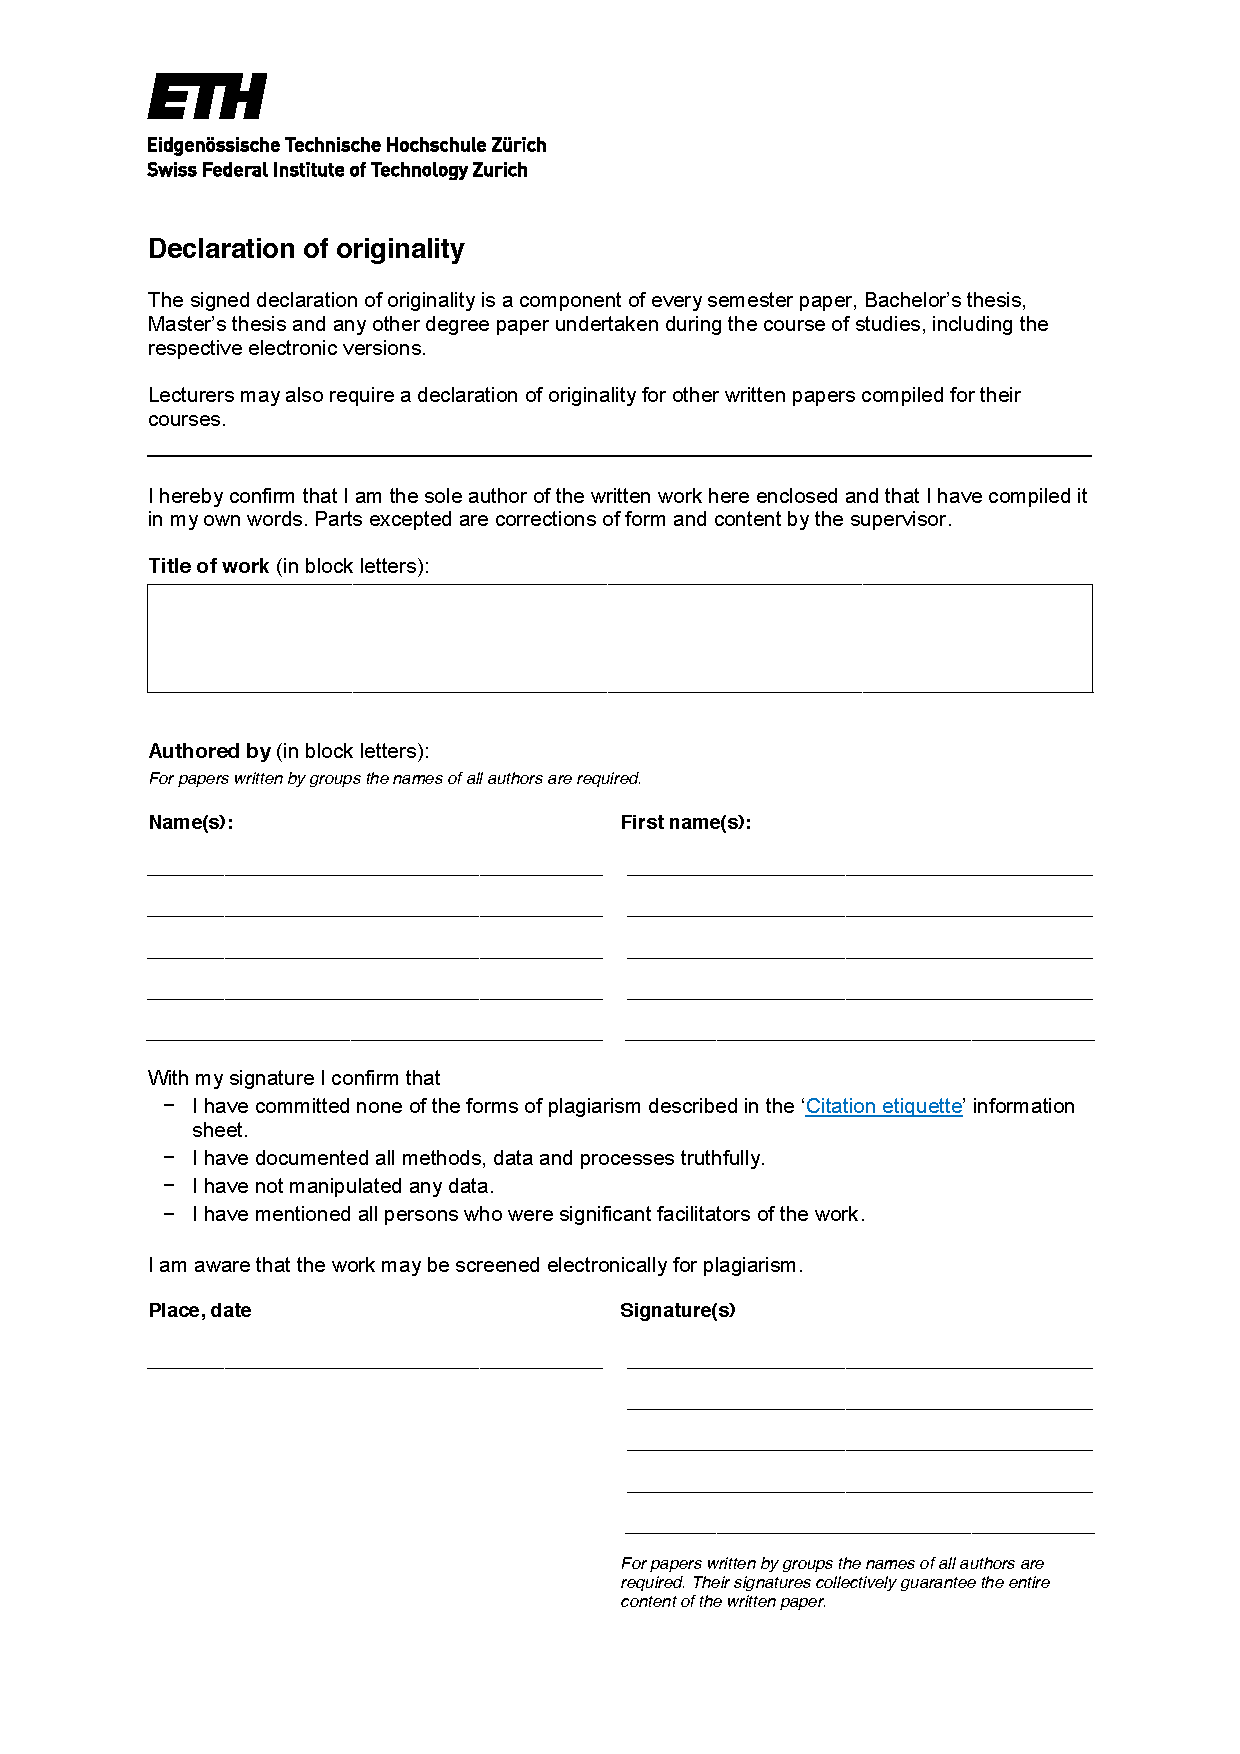
\includepdf[pages={-}]{declaration-originality.pdf}
\end{document}
